\documentclass{book} 

\usepackage{graphicx}
\usepackage{amsmath}
\usepackage{algorithm}
\usepackage{algpseudocode}
\usepackage{float}
\usepackage{hyperref}
\usepackage{placeins}
\usepackage{amssymb}

\usepackage{tikz}
\usetikzlibrary{arrows}
\usetikzlibrary{snakes}
\usetikzlibrary{decorations.pathmorphing}

\hypersetup{
	colorlinks,
	citecolor=black,
	filecolor=black,
	linkcolor=black,
	urlcolor=black
}

\title{Solutions of Introduction to Algorithms}
\author{Saman Saadi}
\date{} 

\begin{document}
	\frontmatter
	\maketitle
%	\newpage
	\tableofcontents
	\mainmatter
	\chapter{Dynamic Programming}
	\section{Rod cutting}
	\paragraph{Proof of the number of cuts}
	Imagine for the rod of size $n$ we have $n$ cuts of length $1$. We assign numbers $1, 2, \dots, n$ to these cuts of length $1$. For $n = 3$ we can have
	\begin{table}[H]
		\centering
		\begin{tabular}{r c c c c c}
			1: & 1 & * & 2 & * & 3 \\
			2: & 1 & * & 2 & & 3 \\
			3: & 1 &  & 2 & * & 3 \\
			4: & 1 & & 2 &  & 3 \\
		\end{tabular}
	\end{table}
	So for a rod of length $n$ we can have at most $n-1$ stars (cuts). Each of these stars can appear or disappear. So the number of ways to cut the rod is $2^{n - 1}$.
	\paragraph{Exercise 2}
	No it cannot always produce an optimal solution. Consider the following example.
	\begin{table}[H]
		\centering
		\begin{tabular}{r||c|c|c}			
			$l_i$ & 1 & 2 & 3\\
			\hline
			$p_i$ & 1 & 50 & 72 \\
			\hline
			$\frac{p_i}{l_i}$ & 1 & 25 & 24
		\end{tabular}
	\end{table}
	For n = 3 the greedy approach cut the rod in 2 pieces. The length of one of them is 2 and the other's is 1. So the profit is $50\$ + 1\$ = 51\$$. But the optimal solution is to keep the rod intact so the profit is $72\$$.
	\paragraph{Exercise 3}
	We can keep the rod intact so we don't need to incur the fixed cost c or we can have at least one cut. We need to choose the best solution among all of them:
	\begin{equation*}
	r(i) = \begin{cases}
	\max\limits_{1 \leq k < n}(p_i, r(i - k) + p_k - c) & i > 0 \\
	0 & i = 0
	\end{cases}
	\end{equation*}
	So the solution is $r(n)$. We have n distinct subproblem. In each step we need to choose between keeping the rod intact or have at least one cut which divide the rod into two pieces. The length of one of them is k and the other's $n - k$. We don't know the exact value of k so we need to try all possible values. This can be done in $O(n)$. Therefore the overall running time is $O(n^2)$
	
	\begin{algorithm}
		\begin{algorithmic}[1]
			\Function{f}{p, n, c}
			\State let r[0..n] be a new array
			\State $r[0] \gets 0$
			\For{$\text{j from 1 to n}$}
			\State $q \gets p[j]$
			\For{i from 1 to $j - 1$}
			\State $q = max(q, r[j - i] + p[i] - c)$
			\EndFor
			\State r[j] = q
			\EndFor
			\State \Return $r[n]$
			\EndFunction
		\end{algorithmic}
	\end{algorithm}
	\section{Matrix-chain multiplication}
	\paragraph{Exercise 4}
	I've used the following equations:
	\begin{align}
	\sum_{i = 1}^{n} i &= \frac{n(n + 1)}{2}\\
	\sum_{i = 1}^{n} i^2 &= \frac{n(n + 1)(2n + 1)}{6}
	\end{align}
	Each node of the graph represents a distinct sub-problem. Suppose we have two nodes v and u. There is an edge from v to u, if the solution of subproblem v is depended on subproblem u. In other words, there is an edge from m[i, j] to all m[i, k] and m[k + 1, j] for $i \le k < j$. \\
	Usually $|V|$ determines space complexity and $|V| + |E|$ time complexity. we know for every subprobelm m[i, j], $j \ge i$. Hence we have $n - i + 1$ subproblems which starts with $A_i$. So the number of vertices is:
	\begin{equation}
	\begin{split}
	|V| &= \sum_{i = 1}^{n}{n - i + 1} \\
	&= \sum_{i=1}^{n}i \\
	&= \frac{n(n + 1)}{2}
	\end{split}
	\end{equation}
	Hence the space complexity is is $O(n^2)$. We don't use all of the array cells when $j < i$. So we waste $\frac{n^2 - n}{2}$ of allocated array. By analyzing lines 5 - 10 of MATRIX-CHAIN-ORDER pseudocode in the text book we can compute the number of edges.
	\begin{figure}[h!]
	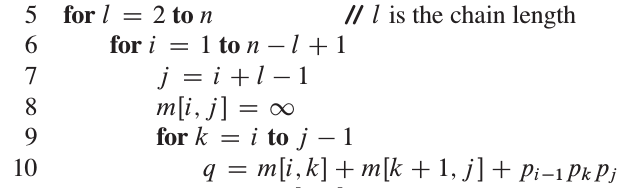
\includegraphics[width=\linewidth]{images/15/15-2-4.png}
	\end{figure}
	As you can see in line 10, m[i, j] is depends on two subproblem m[i, k] and m[k + 1, j]. We visit each distinct subproblem exactly once. So by counting the outdegree of each node we can calculate the number of edges in a directed graph:
	\begin{equation}
	\begin{split}
	|E| &= \sum_{l = 2}^{n}\sum_{i=1}^{n - l + 1}\sum_{k = i}^{i+l-2}2 \\
	&= \sum_{l=2}^{n}\sum_{i=1}^{n-l+1}2(l-1) \\
	&= 2\sum_{l=2}^{n}(n - l + 1)(l-1) \\
	&= 2\sum_{l=2}^{n}(n -(l - 1))(l-1) \\
	&= 2\sum_{l=1}^{n-1}(n-l)l \\
	&= 2(\sum_{l=1}^{n-1}nl - \sum_{l=1}^{n-1}l^2) \\
	&= 2(n\sum_{l=1}^{n-1}l - \sum_{l=1}^{n-1}l^2) \\
	&= 2[n\frac{(n - 1)n}{2} - \frac{(n - 1)(n)(2n - 1)}{6}] \\
	&= n^2(n - 1) - \frac{n(n-1)(2n-1)}{3} \\
	&= \frac{3n^2(n-1)-n(n-1)(2n-1)}{3} \\
	&= \frac{n(n-1)(3n-2n+1)}{3} \\
	&= \frac{n(n-1)(n+1)}{3}\\
	&= \frac{n(n^2-1)}{3}\\
	&= \frac{n^3 - n}{3}
	\end{split}
	\end{equation}
	So the running time is $|V| + |E| = \frac{n^2 + n}{2} + \frac{n^3 - n}{3} = O(n^3)$
	\section{Elements of dynamic programming}
	\paragraph{Exercise 2}
	Each node is filled with (p, r). p is the index of leftmost element and r is the index of rightmost element of array which the subprolem wants to sort. As you can see there is no overlapping between subproblems so dynamic programming is not a good idea for merge sort. In other words, we don't see a previously solved subproblem again and we only waste memory. As a general rule if the subproblem graph is a tree, dynamic programming cannot be applied.
	\begin{figure*}[h!]
		\centering
		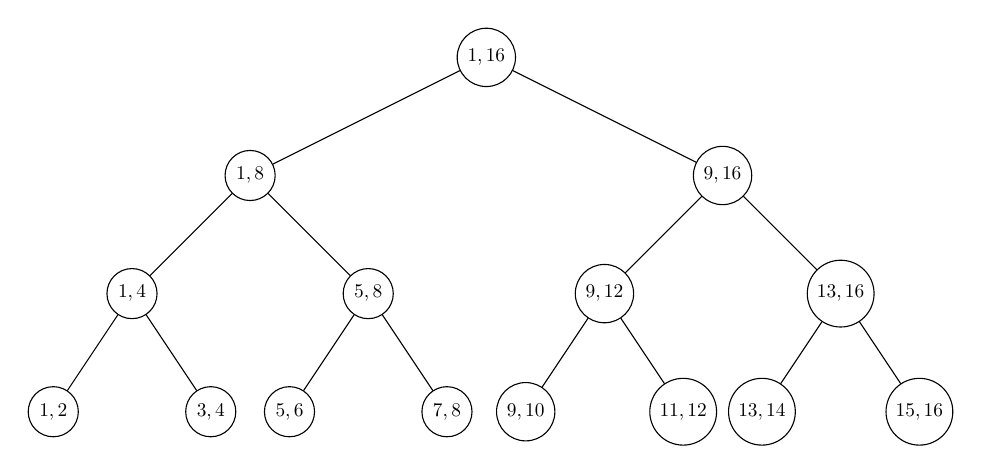
\begin{tikzpicture}[level/.style={sibling distance=60mm/#1}]
		\tikzset{vertex/.style = {shape=circle,draw,scale=0.7}}
			\node[vertex] (a){$1, 16$}
				child {node[vertex] (b) {$1, 8$}
						child {node[vertex] (d) {$1, 4$}
							child {node[vertex] (h) {$1, 2$}}
							child {node[vertex] (i) {$3, 4$}}
							}
						child {node[vertex] (e) {$5, 8$}
							child {node[vertex] (j){$5, 6$}}
							child {node[vertex] (k){$7, 8$}}
							}
					}
				child {node[vertex] (c) {$9, 16$}
					child {node[vertex] (f) {$9, 12$}
						child {node[vertex] (l){$9, 10$}}
						child {node[vertex] (m){$11, 12$}}
						}
					child {node[vertex] (g) {$13, 16$}
						child {node[vertex] (n){$13, 14$}}
						child {node[vertex] (o){$15, 16$}}
						}
					}
				;
		\end{tikzpicture}
	\end{figure*}
	\chapter{Amortized Analysis}
	\section{Aggregate analysis}
	\paragraph{Exercise 1}
	No it doesn't hold. The maximum number of pops, including multipop, is proportional to the number of previous push operations. If we can only push one item, the number of pushed elements is at most $n$. If we add a new operation named multipush, then the number of pushed items is at most $n \times k$. So the amortized cost is $O(k)$. For example we can have two operations. One is multipushing $10^9$ items and the other is multipopping $10^9$ items. It is obvious the total cost is not $O(n) = O(2)$ and is $O(nk) = O(2 \times 10^9)$.
	\paragraph{Exercise 2}
	The following pseudo-code explains how to implement DECREMENT.
	\begin{algorithm*}[h!]
		\begin{algorithmic}[1]
			\Function{DECREMENT}{A}
			\State $i = 0$
			\While{$i < A.length \text{ and } A[i] == 0$}
			\State $A[i] = 1$
			\State $i = i + 1$
			\EndWhile
			\If{$i < A.length$}
			\State $A[i] = 0$
			\EndIf
			\EndFunction
		\end{algorithmic}
	\end{algorithm*}
	The worst case happens when we start with 0 and then decrements it to get $2^k - 1$ which all bits are set to 1 and then increments it to get 0. We repeat this loop until we have n operations. For $n = 4$ and $k = 3$ we have:
	\begin{align*}
		&000 \\
		&111 \\
		&000 \\
		&111
	\end{align*}
	\section{The accounting method}
	For another example of "the accounting method" see exercise 5 of \ref{sec:Representation of graphs}.
	\chapter{Elementary Graph Algorithms}
	\section{Representation of graphs}
	\label{sec:Representation of graphs}
	\paragraph{Exercise 1}
	We know that $adj[u]$ is a list. Depends on the list implementation, it can take $O(1)$ to determine its size. In that case the running time for finding the out-degree of each vertex is $O(V)$. If we cannot determine size of the list in $O(1)$, then the overall running time of algorithm is $O(V + E)$. \\
	The running time for finding in-degree of each vertex is $O(V + E)$.
	\paragraph{Exercise 3}
	For adjacency-matrix it takes $O(V^2)$ and for adjacency-list it takes $O(V + E)$.
	\begin{algorithm}[h!]
		\caption{$G'$ using adjacency matrix}
		\begin{algorithmic}[1]
			\Function{TransposeGraph}{G}
				\State Let $G'$ be a new graph
				\State $G' \gets G$
				\ForAll{$u \in V$}
					\ForAll{$v \in V$}
						\State $G'.A[v][u] = G.A[u][v]$
					\EndFor
				\EndFor
				\State \Return $G'$
			\EndFunction
		\end{algorithmic}
	\end{algorithm}
	\begin{algorithm*}[h!]
		\caption{$G'$ using adjacency list}
		\begin{algorithmic}[1]
			\Function{TransposeGraph}{G}
				\State Let $G'$ be a new graph
				\State $G'.V = G.V$
				\ForAll{$u \in G.V$}
					\ForAll{$v \in G.Adj[u]$}
						\State $G'.Adj[v].insert(u)$
					\EndFor
				\EndFor
			\EndFunction
		\end{algorithmic}
	\end{algorithm*}
	\FloatBarrier
	\paragraph{Exercise 4}
	We create a new adjacency-list for $G'$ called $adj$. For each vertex $u$ in $G$, suppose $v$ is its neighbor. If $u \ne v$, then $adj[u].insert(v)$ and $adj[v].insert(u)$. If there are multiple edges between $u$ and $v$, we see $v$ as $u$'s neighbor more than once. So if the last element if $adj[v]$ is $u$, it means there are more than one edges between them so we shouldn't insert $v$ again. Traversing $G$ takes $O(V + E)$. Finding out there are more than one edge between two vertices is $O(1)$. So the overall running time is $O(V + E)$. Note that I supposed $G$ is also undirected.
	\begin{algorithm}[h!]
		\begin{algorithmic}[1]
			\Function{f}{G}
			\State $\text{let }G' \text{ be a new graph}$
			\State $G'.V = G.V$
			\ForAll{$u \in G.V$}
				\ForAll{$v \in G.adj[u]$}
					\If{$u \ne v \land G'.adj[v].last() \ne u$}
						\State $G'.adj[v].insert(u)$		
					\EndIf
				\EndFor
			\EndFor
			\State \Return $G'$
			\EndFunction
		\end{algorithmic}
	\end{algorithm}
	\paragraph{Exercise 5}
	The running time of matrix-list implementation is $O(V^3)$. Note that having matrix-list named $A$:
	
	\begin{equation*}
	A^2 = A_{|V| \times |V|} \times A_{|V| \times |V|}
	\end{equation*}
	Suppose $a_{ij} \in A$ and $a^2_{ij} \in A^2$ and $a_{ii} = 1$:
	\begin{equation*}
	a^2_{ij} = \sum_{k = 1}^{|V|}{a_{ik} \times a_{kj}}
	\end{equation*}
	So if $a^2_{ij} > 0$ there is at least one path with at most 2 edges between $i$ and $j$. So we can use Strassen multiplication algorithm in $O(n^{2.807})$. But here we use $O(V^3)$ straightforward algorithm.
	 \par For analyzing the running time of adjacency-list implementation we can use amortized analysis.
	\begin{enumerate}
		\item $\boldsymbol{in_u:}$ The number of edges that enter $u$
		\item $\boldsymbol{out_u:}$ The number of edges that leave $u$
		\item $\boldsymbol{(u, v):}$ And edge from u to v $v \ne u$
		\item $\boldsymbol{c_u:}$ The number of times we visit vertex $u$ with at most one edge
		\item $\boldsymbol{c_{(u, v)}:}$ The number of times we visit vertex $v$ with exactly two edges $(x_i, u)$ and $(u, v)$ in which $x_i \in in_u$.
		\item So we visit each vertex $u$ no more than $c_u + \sum_{x \in in_u} {c_{(x, u)}}$.
	\end{enumerate}
	We assign to each vertex $u$ cost $c_u = 1 + in_u$. $1$ is for line \ref{MakeSquareGraph:all_verticies} and $in_u$ is for line \ref{MakeSquareGraph:1-path}. For lines (\ref{MakeSquareGraph:2-path:1} - \ref{MakeSquareGraph:2-path:2}) we assign to each edge cost $c_{(u, v)} = in_u$. So the running time of algorithm, the total number of times we visit each vertex, is $\sum_{u \in V} c_u + \sum_{(u, v) \in E}{c_{(u, v)}}$. We calculate each of them separately. We know the following facts:
	\begin{equation*}
	\begin{split}
		\sum_{u \in V}{in_u} &= |E| \\
		\sum_{u \in V}{out_u} &= |E| \\
		\sum_{(u, v) \in E}{in_u} &= \sum_{u \in V}{in_u \times out_u} \\
		\sum_{(u, v) \in E}{in_u} &\le \sum_{(u, v) \in E}{|V| - 1} \\
		&= |E| \times (|V| - 1)
	\end{split}	
	\end{equation*}
	So we calculate each of the costs separately:
	\begin{equation*}
		\begin{split}
		\sum_{u \in V}{c_{u}} &= \sum_{u \in V}{1 + in_u} \\
		&= \sum_{u \in V}{1} + \sum_{u \in V}{in_u} \\
		&= |V| + |E|
		\end{split}
	\end{equation*}
	and for the last part:
	\begin{equation*}
		\begin{split}
		\sum_{(u, v) \in E}{c_{(u, v)}}  &= \sum_{(u, v) \in E}{in_u} \\
		&\le \sum_{(u, v) \in E}{|V|} \\
		&= |V| \times |E|
		\end{split}
	\end{equation*}
	So the running time of algorithm is $O(|V| + |E| + |V| \times |E|) = O(|V| + |E| \times (1 + |V|)) = O(|V| + |V| \times |E|) = O(|V| \times (1 + |E|)) = O(|V| \times |E|)$.
	\begin{algorithm*}[h!]
		\caption{Finding square graph using matrix-list}
		\begin{algorithmic}[1]
			\Function{MakeSquareGraph}{G}
				\State Let $G'$ be a new Graph
				\Comment $G.A[1..|V|, 1..|V|]$
				\ForAll{$u \in G.V$}
					\ForAll{$v \in G.V$}
						\State $G'.A[u][v] = G.A[u][v]$
						\Comment 1-edge paths
						\If{$G.A[u][v] = 1$}
							\ForAll{$k \in G.V$}
								\State $G'.A[u][k] = G.A[v][k]$
								\Comment 2-edge paths
							\EndFor
						\EndIf
					\EndFor
				\EndFor				
			\EndFunction
		\end{algorithmic}
	\end{algorithm*}
	\begin{algorithm*}[h!]
		\caption{Finding square graph using adjacency-list}
		\begin{algorithmic}[1]
			\Function{MakeSqureGraph}{G}
				\State Let $G'$	be a new graph
				\State $G'.V = G.V$
				\ForAll{$u \in G.V$}
				   \label{MakeSquareGraph:all_verticies}
					\ForAll{$v \in G.Adj[u]$}
						\State $G'.Adj[u].insert(v)$ \label{MakeSquareGraph:1-path}
						\Comment 1-edge paths
						\ForAll{$w \in G.Adj[v]$}		\label{MakeSquareGraph:2-path:1}
						\If {$w \notin G'.Adj[u]$}
							\State $G'.Adj[u].insert(w)$ \label{MakeSquareGraph:2-path:2}
							\Comment 2-edge paths
						\EndIf
						\EndFor						
					\EndFor
				\EndFor
			\EndFunction
		\end{algorithmic}
	\end{algorithm*}
	\FloatBarrier
	\paragraph{Exercise 6}
	Suppose $A$ is an adjacency matrix for $G$.
	\begin{equation*}
		A[i, j] = \begin{cases}
		1 & \text{i cannot be a universal sink} \\
		0 & \text{j cannot be a universal sink}
		\end{cases}
	\end{equation*}
	The following algorithm find the universal sink in $O(V)$. In each step we remove one vertex from all candidates for "universal sink". It takes $O(V)$ to have only one candidate. To determine that candidate is indeed a universal sink we need $O(2V)$ operations. So the overall running time of algorithm is $O(V) + O(2V) = O(V)$.
	\begin{algorithm*}[h!]
		\begin{algorithmic}[1]
			\Function{getUniversalSink}{G}
				\State $A = G.A$
				\Comment $A[1..|V|, 1..|V|]$
				\State $u \gets 1$								
				\While{$u \le |V|$}
					\State $v \gets u + 1$
					\State $sink \gets u$
					\Comment Vertices from $sink$ to $|V|$ can be universal sink					
					\While{$v \le |V| \land A[u, v] = 0$}
						\State $v \gets v + 1$
						\Comment $v$ cannot be a universal sink
					\EndWhile
					\State $u \gets v$
					\Comment $u$ to $v - 1$ cannot be a universal sink
				\EndWhile
				\For{$c$ from $1$ to $sink - 1$}
					\If{$A[sink, c] \ne 0$}
						\State \Return "No universal sink"
					\EndIf
				\EndFor
				\For{$r \in V - \{sink\}$}
					\If{$A[r, sink] \ne 1$}
						\State \Return "No universal sink"
					\EndIf
				\EndFor
				\State \Return sink
			\EndFunction
		\end{algorithmic}
	\end{algorithm*}
	\FloatBarrier
	\paragraph{Exercise 7}
	We know that $B$ is an $|V| \times |E|$ matrix which we show it as $B_{|V| \times |E|}$. By definition $B^T$ is an $|E| \times |V|$ matrix which we show it as $B_{|E| \times |V|}^T$. We define $P_{|V| \times |V|} = B_{|V| \times |E|} \times B_{|E| \times |V|}^T$.
	\begin{equation*}	
	\begin{split}
		p_{ij} &= \sum_{e \in E}b_{ie} \times b^T_{ej} \\
		&= \sum_{e \in E}b_{ie} \times b_{je}
	\end{split}
	\end{equation*}
	
	There are two cases:
	\begin{enumerate}
		\item $\boldsymbol{i \ne j:}$
			\begin{equation*}
			b_{ie} \times b_{je} = \begin{cases}
			-1 \times 1 & e = (i, j) \in E \\
			1 \times -1 & e = (j, i) \in E \\
			0 & otherwise
			\end{cases}
			\end{equation*}
			
			So $p_{ij}$ is the number of edges between $i$ and $j$.
			
		\item $\boldsymbol{i = j:}$
		
			\begin{equation*}
			b_{ie} \times b_{je} = b_{ie} \times b_{ie} = \begin{cases}
			-1 \times -1 & e = (i, j) \in E \land j \ne i \\
			1 \times 1 & e = (j, i) \in E \land j \ne i \\
			0 \times 0 & otherwise
			\end{cases}
			\end{equation*}
			
			In this case $p_{ii}$ is the sum of all edges that enter and leave the vertex $i$.		
	\end{enumerate}
	We can summarize the answer
	\begin{equation*}
		p_{ij} = \begin{cases}
		-|S| \text{ such as } S = \{e \in E : e = (i, j) \lor e = (j, i)\} & i \ne j \\
		indegree(i) + outdegree(i) & i = j
		\end{cases}
	\end{equation*}
	
	\section{Breadth-first search}
	\label{psec:BFSAlgorithm}
	\paragraph{BFS algorithm}
	For understanding the following algorithm see Lemma 22.3 from the textbook.
	
	\textbf{Lemma 22.3: } Suppose that during the execution of BFS on graph G = (V, E), the queue Q contains the vertices $[v_1, v_2, \dots , v_r]$, where $v_1$ is the head of Q and $v_r$ is the tail. Then $v_r.d \le v_1.d$ and $v_i.d \le v_{i+1}.d$ for $i = 1, 2, \dots, r - 1$.\\
			
	As you can see $(u, v)$ cannot be a forward edge (u is the ancestor of v) in BFS algorithm. \\
	
	\textbf{Proof:} Suppose in BFS first we discover $u$ and $(u, v) \in E$ and $w$ is reachable from $u$. The shortest path from $u$ to $w$ is $\{v_1, v_2, \dots, v_k\}$ for $k > 2$. See figure \ref{fig:No forward edge in BFS}. In order $(u, v)$ be a forward edge, we must discover $w$ before $v$. According to BFS properties it's $v$ which is discovered first.
	
	\begin{figure}[h!]
		\centering
		\caption{No forward edge in BFS}
		\label{fig:No forward edge in BFS}
		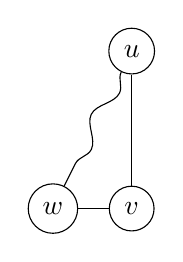
\begin{tikzpicture}
		\tikzset{vertex/.style={shape = circle, draw, minimum size = 1.5em}}
		\tikzset{snake it/.style={
				decoration={snake, 
					amplitude = 1mm,
					segment length = 8mm,
					post length=0.9mm},decorate}}
		%vertices
		\node[vertex] (u) at (1, 2) {$u$};
		\node[vertex] (w) at (0, 0) {$w$};
		\node[vertex] (v) at (1, 0) {$v$};
		%edges
		\path (u) edge[snake it] (w);
		\path (w) edge (v);
		\path (u) edge (v);
		\end{tikzpicture}
	\end{figure}
	
	\begin{algorithm*}[h!]
		\caption{BFS algorithm}
		\begin{algorithmic}
			\Statex
		\end{algorithmic}
		\begin{algorithmic}[1]		
			\Function{BFS}{G, s}
				\ForAll{$u \in G.V - \{s\}$}
					\State $u.color = WHITE$
					\State $u.d = \infty$
					\State $u.\pi = NIL$
				\EndFor
				\State $s.color = GRAY$
				\State $s.d = 0$
				\State $s.\pi = NIL$
				\State $Q = \emptyset$
				\State \Call{Enqueue}{Q, s}
				\While{$Q \ne \emptyset$}
					\State $u = $ \Call{Dequeue}{Q}
					\ForAll{$v \in G.adj[u]$}
						\If{$v.color == WHITE$} \Comment edge $(u, v)$ is a tree edge
							\State $v.color = GRAY$
							\State $v.d = u.d + 1$
							\State $v.\pi = u$
							\State \Call{Enqueue}{Q, v}
						\ElsIf{u.d == v.d + 1} \Comment back edge
							\State \Call{Assert}{$v.color == BLACK$}						
						\ElsIf{v.d == u.d + 1} \Comment cross edge
							\State \Call{Assert}{$v.color == GRAY$}
						\ElsIf{u.d == v.d} \Comment cross edge
							\State \Call{Assert}{$v.color == GRAY$}

						\EndIf
					\EndFor
					\State $u.color = BLACK$
				\EndWhile
			\EndFunction
		\end{algorithmic}				
	\end{algorithm*}		
	\FloatBarrier
	
	\label{psec:BFScharacteristics}
	\paragraph{BFS characteristics}
	\begin{itemize}
		\item Note that in BFS if $(u, v)$ is a back edge (v is the ancestor of u in BFS tree), then the color of v is black (in DFS it's gray). As you can see in figure \ref{fig:BackEdgeInBfs}, BFS starts from $v$ and when we navigate edge $(u, v)$ the color of $v$ is black. In other words $w.d = v.d + 1 \land u.d = w.d + 1$.
		
		\begin{figure*}[h!]
			\centering
			\caption{Back edge in BFS}
			\label{fig:BackEdgeInBfs}
			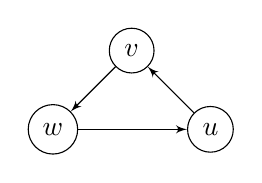
\begin{tikzpicture}
			\tikzset{vertex/.style={shape = circle, draw, minimum size = 1.5em}}
			\tikzset{edge/.style={->, > = latex'}}
			\tikzset{snake it/.style={-stealth,
					decoration={snake, 
						amplitude = 1mm,
						segment length = 8mm,
						post length=0.9mm},decorate}}
			%vertices
			\node[vertex] (w) at (0, 0) {$w$};
			\node[vertex] (u) at (2, 0) {$u$};
			\node[vertex] (v) at (1, 1) {$v$};
			%edges
  			\draw[edge] (v) -- (w);
  			\draw[edge] (w) -- (u);
			\draw[edge] (u) -- (v);
			\end{tikzpicture}
		\end{figure*}
		\FloatBarrier

		\item If the graph is undirected, after running BFS algorithms, for all back edges $(u, v)$, $v$ is the parent of $u$.				
		\item If $(u, v)$ is a cross edge, the color of $v$ can be gray. Unlike DFS in which the color of $v$ is always black.
		
		\item In BFS both directed and undirected graphs can have cross edges.
		
		\item If the graph is undirected, a cross edge in BFS means we have an undirected cycle in graph.
		
		\item Since in an undirected graph $(u, v) \in E$ means $(v, u) \in E$, we always have back edges. In other words for all tree edges $(u, v)$, $(v, u)$ is a back edge. This is true for both BFS and DFS algorithms.
		
		\item It's easier to use BFS for finding cycles in undirected graphs which takes $O(V + E)$. If we encounter a cross edge, we have a cycle. If we want a faster approach for undirected graph, we need to use DFS which takes $O(V)$. for more information see exercise 3 of Topological sort. For directed graphs, it's better to use DFS. If we have a back edge, it means we have a cycle. If you want to use DFS for undirected graph see \textbf{Exercise 10 of DFS}.
	 
	\end{itemize}

    \phantomsection
    \label{psec:bfs_exercise_7}
	\paragraph{Exercise 7}
	For another good example see "Find the number of shortest path between" on \ref{psec:ShortestPathClassification}. We need to determine whether an undirected graph is bipartite or not. We can paint the vertices of a bipartite graph with two colors in such a way that no two adjacent vertices share the same color.\\
	We can easily prove that if there is a cycle in graph in which the number of edges is odd, then the graph cannot be bipartite. \\
	We can use BFS. We know that in BFS algorithm we can only have tree and back and cross edges (see \ref{psec:BFSAlgorithm}). Note that in BFS we can have cross edges whether or not the graph is directed. We run BFS on an arbitrary vertex $s$. Suppose $u$ is reachable from $s$. If $u.d$ is even we color that vertex "blue" otherwise we color it "red". For tree edges we don't have any problem. Since in back edges in BFS there is a parent-child relationship between two vertices of an endge, we don't have any problem with back edges. We need to think about cross edges. We know that $\delta(s, u) = u.d$ which is the shortest path from $s$ to $u$. \\
	
			\begin{figure}[h!]
				\centering
				\caption{DFS tree}
				\label{fig:DFS tree}
				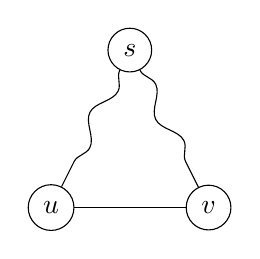
\begin{tikzpicture}
				\tikzset{vertex/.style={shape = circle, draw, minimum size = 1.5em}}
				\tikzset{snake it/.style={
						decoration={snake, 
							amplitude = 1mm,
							segment length = 8mm,
							post length=0.9mm},decorate}}
				%vertices
				\node[vertex] (s) at (1, 2) {$s$};
				\node[vertex] (u) at (0, 0) {$u$};
				\node[vertex] (v) at (2, 0) {$v$};
				%edges
				\path (s) edge[snake it] (u);
				\path (s) edge[snake it] (v);
				\path (u) edge (v);
				\end{tikzpicture}
			\end{figure}
			
	\textbf{Lemma 22.3: } Suppose that during the execution of BFS on graph G = (V, E), the queue Q contains the vertices $[v_1, v_2, \dots , v_r]$, where $v_1$ is the head of Q and $v_r$ is the tail. Then $v_r.d \le v_1.d$ and $v_i.d \le v_{i+1}.d$ for $i = 1, 2, \dots, r - 1$.\\
	
	For more information about Lemma 22.3 see the textbook. Suppose $Q = \{v_1, v_2, \dots , v_r\}$ as we defined it in Lemma 22.3. Note that if we encounter a cross edge, it connects two vertices (u, v) that $u \in Q \land v \in Q$. To be more specific, first we pop $u$ from queue and then we find out $(u, v)$ is a cross edge. In that moment $u \notin Q \land v \in Q$.\\
	
	Suppose $(u, v)$ is not a tree edge (since the graph is undirected, it's a cross edge). An upper bound for $u.d$:
	
	\begin{equation*}
	u.d \le v.d + 1 \Rightarrow u.d - v.d \le 1
	\end{equation*}
	
	On the other hand an upper bound for $v.d$ (note that the graph is undirected):
	
	\begin{equation*}
	v.d \le u.d + 1 \Rightarrow v.d - u.d \le 1
	\end{equation*}
	
	So we can say:
	
	\begin{equation*}
		|u.d - v.d| \le 1 \Rightarrow -1 \le u.d - v.d \le 1
	\end{equation*}
	
	If $|u.d - v.d| = 1$, then $u$ and $v$ have different colors. So we only need to consider $u.d = v.d$. In that case both $u$ and $v$ have the same color and we need to prove that this graph cannot be bipartite. When we have a cross edge in an undirected graph, it means that we have a cycle (see figure \ref{fig:DFS tree}). The number of edges in this cycle is $u.d + v.d + 1 = 2 \times u.d + 1$ which is odd. So the graph cannot be bipartite. Note that the graph can have more than one connected component so it is possible we need to run BFS more than once.
	\begin{algorithm*}[h!]
		\caption{Determining whether a graph is bipartite or not}
		\begin{algorithmic}[1]
			\Function{IsBipartiteGraph}{G}
				\ForAll{$u \in G.V$}
					\State $u.color = WHITE$
					\State $u.d = \infty$
					\State $u.\pi = NIL$
				\EndFor
				\ForAll{$u \in G.V$}
					\If{$u.color == WHITE\text{ }\land$ \Call{BFS}{G, u}$\text{ } == FALSE$}
						\State \Return $FALSE$
					\EndIf
				\EndFor	
				\State \Return $TRUE$
			\EndFunction		
		\end{algorithmic}
		\begin{algorithmic}
			\Statex
		\end{algorithmic}
		\begin{algorithmic}[1]		
			\Function{BFS}{G, s}
				\State $s.color = GRAY$
				\State $s.d = 0$
				\State $Q = \emptyset$
				\State \Call{Enqueue}{Q, s}
				\While{$Q \ne \emptyset$}
					\State $u = $ \Call{Dequeue}{Q}
					\ForAll{$v \in G.adj[u]$}
						\If{$v.color == WHITE$} \Comment edge $(u, v)$ is a tree edge
							\State $v.color = GRAY$
							\State $v.d = u.d + 1$
							\State $v.\pi = u$
							\State \Call{Enqueue}{Q, v}
						\ElsIf{u.d == v.d}
							\State \Return $FALSE$
						\EndIf
					\EndFor
					\State $u.color = BLACK$
				\EndWhile
				\State \Return $TRUE$
			\EndFunction
		\end{algorithmic}				
	\end{algorithm*}
	\FloatBarrier
	\paragraph{Exercise 8}
	Suppose the maximum distance is path $p = (v_0, v_1, \dots, v_k)$ in which $u = v_0$ and $v = v_k$. Consider an arbitrary vertex $s$. We know that there is exactly one path between every two vertices in a tree. We have two cases.
	\begin{enumerate}
		\item $\boldsymbol{s \in p}$
		\begin{figure}[h!]
			\centering
			\caption{$s \in p$}
			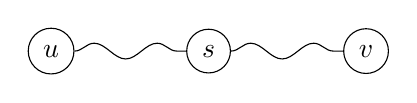
\begin{tikzpicture}
			\tikzset{vertex/.style={shape = circle, draw, minimum size = 1.5em}}
			\tikzset{snake it/.style={
					decoration={snake, 
						amplitude = 1mm,
						segment length = 8mm,
						post length=0.9mm},decorate}}
			%vertices
			\node[vertex] (u) at (0, 0) {$u$};
			\node[vertex] (s) at (2, 0) {$s$};
			\node[vertex] (v) at (4, 0) {$v$};
			%edges
			\path (u) edge[snake it] (s);
			\path (s) edge[snake it] (v);
			\end{tikzpicture}
		\end{figure}		
		\item $\boldsymbol{s \not \in p:}$ In this case there is exactly one path between $s$ and $w \in p - \{u\} - \{v\}$. For example if $w = u$ then the diameter is between $s$ and $v$.
		\begin{figure}[h!]
			\centering
			\caption{$s \not\in p \land w \in p - \{u\} - \{v\}$}
			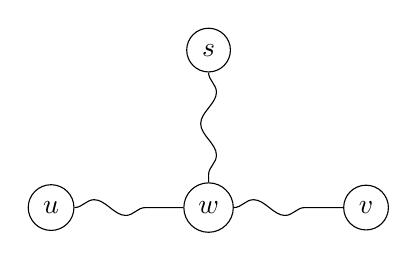
\begin{tikzpicture}
			\tikzset{vertex/.style={shape = circle, draw, minimum size = 1.5em}}
			\tikzset{snake it/.style={
					decoration={snake, 
						amplitude = 1mm,
						segment length = 8mm,
						post length=0.9mm},decorate}}
			%vertices
			\node[vertex] (u) at (0, 0) {$u$};
			\node[vertex] (w) at (2, 0) {$w$};
			\node[vertex] (v) at (4, 0) {$v$};
			\node[vertex] (s) at (2, 2) {$s$};
			%edges
			\path (u) edge[snake it] (w);
			\path (w) edge[snake it] (v);
			\path (s) edge[snake it] (w);			
			\end{tikzpicture}
		\end{figure}		
	\end{enumerate}
	If we run BFS on $s$, then $\max\limits_{x \in G.V}(x.d)$ belongs to either $u$ or $v$. Otherwise the diameter is not between $u$ and $v$. Without loss of generality suppose it is $u.d = \max\limits_{x \in G.V}(x.d)$. Then we run another BFS on $u$ to get $v$ in a similar manner. The running time of algorithm is $O(2V + 2E) = O(V + E)$. Since in a tree $|E| = |V| - 1$ the running time is $O(V)$.
	\begin{algorithm}[h!]
		\begin{algorithmic}[1]
			\Function{FindDiameter}{G}
			\State Let $s$ be an arbitrary vertex such that  $s \in G.V$
			\State \Call{InitBFS}{G}
			\State u = \Call{BFS}{G, s}
			\State \Call{InitBFS}{G}
			\State v = \Call{BFS}{G, u}
			\State \Return $u, v, v.d$
			\EndFunction
		\end{algorithmic}
	\end{algorithm}
	\begin{algorithm}[h!]		
		\begin{algorithmic}[1]
			\Function{BFS}{G, s}			
				\State $s.color = GRAY$
				\State $s.d = 0$
				\State $Q = \emptyset$
				\State \Call{Enqueue}{Q, s}
				\State $max = -\infty$
				\While{$Q \ne \emptyset$}
					\State $u = $ \Call{Dequeue}{Q}
					\ForAll{$v \in G.adj[u]$}
						\If{$v.color == WHITE$}
							\State $v.color = GRAY$
							\State $v.d = u.d + 1$
							\If{$v.d > max$}
								\State $max = v.d$
								\State $z = v$
							\EndIf
							\State $v.\pi = u$
							\State \Call{Enqueue}{Q, v}
						\EndIf
					\EndFor
					\State $u.color = BLACK$
					\EndWhile
					\State \Return $z$
			\EndFunction																				
		\end{algorithmic}	
	\end{algorithm}
	\FloatBarrier	
	\paragraph{exercise 9}
	This undirected graph is equivalent to a directed graph which for all $u, v \in V$, $(u, v), (v, u) \in E$. We can use a modified version of DFS. Because we have both edges $(u, v)$ and $(v, u)$, we don't have "cross edges". We need to choose between "forward edges" or "back edges". In the following algorithm we use "forward edges" and skip "back edges".
	\begin{algorithm*}
		\begin{algorithmic}[1]
			\Function{DFS}{G, u}
				\State $u.color \gets Gray$
				\State $paths \gets \phi$
				\ForAll{$v \in G.Adj[u]$}
					\If{$v.color = White$} \Comment{Tree edge}
						\State $paths \gets \{(u, v)\} \cup DFS(G, v) \cup \{(v, u)\}$
					\ElsIf{$v.color = Black$} \Comment{Forward edge}
						\State $paths \gets paths \cup \{u, v\} \cup \{v, u\}$
					\EndIf
				\EndFor
				\State $u.color \gets Black$
				\State \Return paths
			\EndFunction
		\end{algorithmic}
	\end{algorithm*}
	\FloatBarrier
	\section{Depth-first search}
	\phantomsection
	\label{psec:EdgeClassification}
	\paragraph{Edge classification}
	\begin{itemize}
	\item[\textbf{Tree edges}] are edges in the depth-first forest $G_\pi$. Edge $(u, v)$ is a tree edge if v was discovered by exploring edge $(u, v)$
	\item[\textbf{Back edges}] are those edges $(u, v)$ connecting a vertex $u$ to \textbf{an ancestor} $v$ in a depth-first tree. We consider self-loops, which may occur in directed graphs, to be back edges.\\
	Note that a directed graph is acyclic if and only if a depth-first search yields no back edges.\\
	
	Undirected graphs are tricky. Since $(u, v) \in E \land (v, u) \in E$, $(u, v)$ is a back edge if and only if $(v, u)$ is a tree edge.
	\item[\textbf{Forward edges}] are those nontree edges $(u, v)$ connecting a vertex $u$ to a descendant $v$ in a depth-first tree.
	\item[\textbf{Cross edges}] are all other edges. They can go between vertices in the same depth-first tree, as long as one vertex is not an ancestor of the other, or they can go between vertices in different depth-first trees.
	\end{itemize}
	The DFS algorithm has enough information to classify some edges as it encounters them. The key idea is that when we first explore an edge $(u, v)$, the color of vertex $v$ tells us something about the edge:
	\begin{enumerate}
	\item \textbf{WHITE} indicates a \textbf{tree} edge
	\item \textbf{GRAY} indicates a \textbf{back} edge
	\item \textbf{BLACK} indicates a \textbf{forward or cross} edge. It's \textbf{forward} edge If $u.d < v.d$ and it's \textbf{cross} edge if $u.d > v.d$.
	\end{enumerate}
	Suppose $s$ is the root of DFS or BFS tree.
	\begin{itemize}
		\item \textbf{Tree edge}
		\begin{itemize}
			\item Directed graph
			\begin{itemize}
				\item DFS: We can have tree edges
				\item BFS: We can have tree edges
			\end{itemize}
			\item Undirected graph
			\begin{itemize}
				\item DFS: We can have tree edges
				\item BFS: We can have tree edges
			\end{itemize}				
		\end{itemize}
		\item \textbf{Forward edge}
		\begin{itemize}
			\item Directed graph
			\begin{itemize}
				\item DFS: We can have forward edges
				\item BFS: We can't have forward edges. Refer to the beginning of chapter \ref{psec:BFSAlgorithm}
			\end{itemize}
			\item Undirected graph
			\begin{itemize}
				\item DFS: We can't have forward edges
				\item BFS: We can't have forward edges
			\end{itemize}				
		\end{itemize}
		\item \textbf{Back edge}
		\begin{itemize}
			\item Directed graph
			\begin{itemize}
				\item DFS: We can have back edges
				\item BFS: We can have back edges. See problem 22-1 from the textbook.
			\end{itemize}
			\item Undirected graph
			\begin{itemize}
				\item DFS: We can have back edges
				\item BFS: We can have back edges. Suppose $(u, v)$ is a back edge, then $v$ is the parent of $u$ for more information see the beginning of chapter \ref{psec:BFSAlgorithm}.
			\end{itemize}
		\end{itemize}
		\item \textbf{Cross edge}
		\begin{itemize}
			\item Directed graph
			\begin{itemize}
				\item DFS: We can have cross edges
				\item BFS: We can have cross edges. refer to the beginning of chapter \ref{psec:BFSAlgorithm}. For an example see figure \ref{fig:BfsCrossEdgeDirectedGraph}
			\end{itemize}
			\item Undirected graph
			\begin{itemize}
				\item DFS: We can't have cross edges
				\item BFS: We can have cross edges. See the beginning of chapter \ref{psec:BFSAlgorithm}.
			\end{itemize}
		\end{itemize}		
	\end{itemize}
	\begin{figure*}[h!]
		\centering
		\caption{BFS -- cross edge in a directed graph. $v.d \le u.d + 1$}
		\label{fig:BfsCrossEdgeDirectedGraph}
		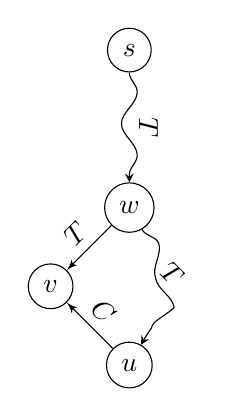
\begin{tikzpicture}
		\tikzset{vertex/.style={shape = circle, draw, minimum size = 1.5em}}
		\tikzset{edge/.style={->, > = latex'}}
		\tikzset{snake it/.style={-stealth,
				decoration={snake, 
					amplitude = 1mm,
					segment length = 8mm,
					post length=0.9mm},decorate}}
		%vertices
		\node[vertex] (s) at (0, 2) {$s$};
		\node[vertex] (w) at (0, 0) {$w$};
		\node[vertex] (u) at (0, -2) {$u$};
		\node[vertex] (v) at (-1, -1) {$v$};
		%edges
		\path[edge] (s) edge[snake it] node[midway, above, rotate=-90]{$T$} (w);
		\path[edge] (w) edge[snake it, bend left] node[midway, above, rotate=-45]{$T$} (u);
		\draw[edge] (w) -- (v) node[midway, above, rotate=45]{$T$};
		\draw[edge] (u) -- (v) node[midway, above, rotate=-45]{$C$};
		\end{tikzpicture}
	\end{figure*}
	\FloatBarrier	
	\paragraph{Exercise 1}
	You can use the following facts. Suppose we have edge (u, v) and we consider loops as back edges (If back edge is a loop then $v.d = u.d \land v.f = u.f$).
	\begin{align*}	
	\begin{split}
		\text{\textbf{Tree edge: }} u.d &< v.d < v.f < u.f \\
		\text{\textbf{Forward edge: }} u.d &< v.d < v.f < u.f \\
		\text{\textbf{Back edge: }} v.d &\le u.d < u.f \le v.f \\
		\text{\textbf{Cross edge: }} v.d &< v.f < u.d < u.f \\
	\end{split}
	\end{align*}
	Note that when the graph is undirected we don't have "forward edge" and "cross edge". Because they are equivalent to "back edge" and "tree edge" respectively.
	\begin{table*}[h!]
		\centering
		\caption{Directed graph}
		\begin{tabular}{r|c|c|c}
			& white & gray & black \\
			\hline
			white & tree, back, forward, cross & back, cross & cross \\
			\hline
			gray & tree, forward  & tree, back, forward & tree, forward, cross \\
			\hline
			black & impossible & back & tree, back, forward, cross \\
		\end{tabular}
	\end{table*}
	\begin{table*}[h!]
		\centering
		\caption{Undirected graph}
		\begin{tabular}{r|c|c|c}
			& white & gray & black \\
			\hline
			white & tree, back & tree, back & impossible \\
			\hline
			gray & tree, back & tree, back & tree, back\\
			\hline
			black & impossible & tree, back & tree, back \\
		\end{tabular}
	\end{table*}
	\FloatBarrier
	\paragraph{Excercise 8}
	We need to show some examples which there is only one path from $u$ to $v$ and at least of one the edges in this path is non-tree edge. Without loss of generality, suppose in this path except $e = (w, x)$ which is a non-tree edge, all other edges are tree ones. We consider all possible types.
	\begin{figure*}[h!]
		\centering
		\caption{Edge e = (w, x) is a non-tree edge}
		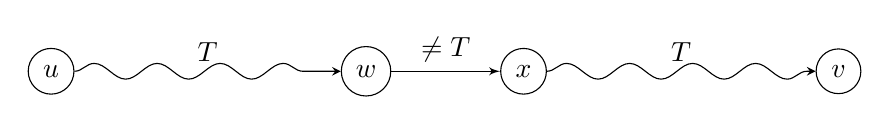
\begin{tikzpicture}
			\tikzset{vertex/.style={shape = circle, draw, minimum size = 1.5em}}
			\tikzset{edge/.style={->, > = latex'}}
		\tikzset{snake it/.style={-stealth,
				decoration={snake, 
					amplitude = 1mm,
					segment length = 8mm,
					post length=0.9mm},decorate}}
			%vertices
			\node[vertex] (u) at (0, 0) {$u$};
			\node[vertex] (w) at (4, 0) {$w$};
			\node[vertex] (x) at (6, 0) {$x$};
			\node[vertex] (v) at (10, 0) {$v$};
			%edges
			\path[edge] (u) edge[snake it] node[midway, above]{$T$} (w);
			\draw[edge] (w) -- (x) node[midway, above]{$\ne T$};
			\path[edge] (x) edge[snake it] node[midway, above]{$T$} (v);
		\end{tikzpicture}
	\end{figure*}
	\begin{itemize}
		\item \textbf{Forward Edge:} If $(w, x)$ is forward ege, then $w$ is an ancestor of $x$ which leads to $v$ be a descendant of $u$. So it cannot be a forward edge
		\item \textbf{Cross edge:} If $(w, x)$ is a cross edge, then $x$ finishes before the discovery of $w$. In other words, all reachable vertices from $x$, including $v$, will be discover before $w$ and $u$. So it cannot be a cross edge
		\item \textbf{Back edge:} Consider the following example which the root of DFS tree is vertex $x$ and it discover $u$ before $v$.
	\begin{figure*}[h!]
		\centering
		\caption{Counterexample using back edge}
		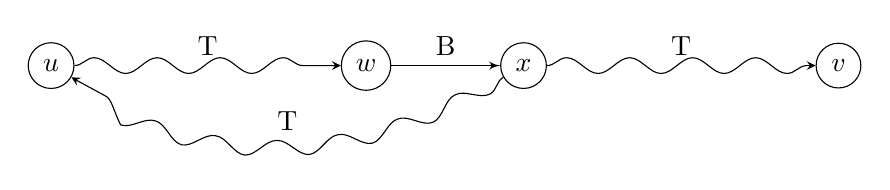
\begin{tikzpicture}
		\tikzset{vertex/.style={shape = circle, draw, minimum size = 1.5em}}
		\tikzset{edge/.style={->, > = latex'}}
		\tikzset{snake it/.style={-stealth,
				decoration={snake, 
					amplitude = 1mm,
					segment length = 8mm,
					post length=0.9mm},decorate}}			
					%vertices
					\node[vertex] (s) at (6, 0) {$x$};
					\node[vertex] (u) at (0, 0) {$u$};
					\node[vertex] (w) at (4, 0) {$w$};
					\node[vertex] (v) at (10, 0) {$v$};
					%edges
					\path[edge] (s) edge[snake it, bend left] node[midway, above] {T} (u);
					\path[edge] (u) edge[snake it] node[midway, above] {T} (w);
					\draw[edge] (w) -- (s) node[midway, above]{B};
					\path[edge] (s) edge[snake it] node[midway, above]{T}(v);
					
					\end{tikzpicture}
					\end{figure*}		
	\end{itemize}
	\FloatBarrier
	\paragraph{Excercise 9}
	Suppose we have edge (u, v) and we consider loops as back edges.
	\begin{align*}	
	\begin{split}
	\text{\textbf{Tree edge: }} u.d &< v.d < v.f < u.f \\
	\text{\textbf{Forward edge: }} u.d &< v.d < v.f < u.f \\
	\text{\textbf{Back edge: }} v.d &\le u.d < u.f \le v.f \\
	\text{\textbf{Cross edge: }} v.d &< v.f < u.d < u.f \\
	\end{split}
	\end{align*}
	We want to find an example in which there is a path from $u$ to $v$ such that $u.f < v.d$. In the path from $u$ to $v$ there should be at least one edge $(w, x)$ which is not a tree edge and $w.f < x.f$ so all ancestors of $w$, including $u$ have a chance to finish before all  descendants of $x$, including $v$. As you can see only back edge has such property. This is like previous example. We start DFS from $x$ and then first visiting u and then finally v. So we have $x.d < u.d < w.d < w.f < u.f < v.d < v.f < x.f$.
	
	\begin{figure*}[h!]
		\centering
		\caption{Counterexample using back edge}
		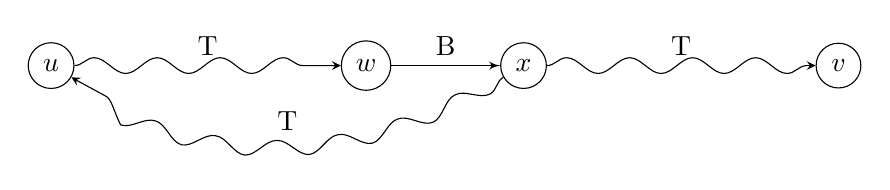
\begin{tikzpicture}
		\tikzset{vertex/.style={shape = circle, draw, minimum size = 1.5em}}
		\tikzset{edge/.style={->, > = latex'}}
		\tikzset{snake it/.style={-stealth,
				decoration={snake, 
					amplitude = 1mm,
					segment length = 8mm,
					post length=0.9mm},decorate}}			
					%vertices
					\node[vertex] (s) at (6, 0) {$x$};
					\node[vertex] (u) at (0, 0) {$u$};
					\node[vertex] (w) at (4, 0) {$w$};
					\node[vertex] (v) at (10, 0) {$v$};
					%edges
					\path[edge] (s) edge[snake it, bend left] node[midway, above] {T} (u);
					\path[edge] (u) edge[snake it] node[midway, above] {T} (w);
					\draw[edge] (w) -- (s) node[midway, above]{B};
					\path[edge] (s) edge[snake it] node[midway, above]{T}(v);
					
					\end{tikzpicture}
					\end{figure*}	
	
	\FloatBarrier
	\paragraph{Exercise 10}
	The algorithm for directed graph:
	\begin{algorithm*}
		\begin{algorithmic}[1]
			\Function {DFS-VISIT}{G, u}
				\State $time = time + 1$
				\State $u.d = time$
				\State $u.color = GRAY$
				\ForAll{$v \in G.adj[u]$}
					\If{$v.color == WHITE$} \Comment edge $(u, v)$ is a tree edge
						\State \Call{PRINT-EDGE}{u, v, TREE}
						\State $v.\pi = u$
						\State \Call{DFS-VISIT}{$G, v$}
					\ElsIf{$v.color == GRAY$} \Comment edge $u, v$ is a back edge
						\State \Call{PRINT-EDGE}{u, v, BACK}
					\ElsIf{$u.d < v.d$}
						\State \Call{PRINT-EDGE}{u, v, FORWARD}
					\Else
						\State \Call{PRINT-EDGE}{u, v, CROSS}
					\EndIf
				\EndFor
				\State $u.color = BLACK$
				\State $time = time + 1$
				\State $u.f = time$
			\EndFunction
		\end{algorithmic}
	\end{algorithm*}
	\FloatBarrier
	
	In an undirected graph forward edges are equivalent to back edges and cross edges are equivalent to tree edges. In other words we only have tree and back edges. Another tricky thing that we need to handle: if $(u, v) \in E$ then $(v, u) \in E$. So if we consider $(u, v)$ as a tree edge then $(v, u)$ is a back edge. In most cases this is not desirable. So we assume if $(u, v)$ is a tree edge, then $(v, u)$ is also a tree edge. Another tricky thing is back edges. If $(u, v)$ is a back edge, then $(v, u)$ is also a back edge. When we are visiting edge $(u, v)$ the color of $v$ is GRAY. On the other side when we are visiting edge $(v, u)$ (which is after visiting edge $(u, v)$), the color of $u$ is BLACK.
	
		\begin{algorithm*}
			\begin{algorithmic}[1]
				\Function {DFS-VISIT}{G, u}
					\State $time = time + 1$
					\State $u.d = time$
					\State $u.color = GRAY$
					\ForAll{$v \in G.adj[u]$}
						\If{$v.color == WHITE$} \Comment edge $(u, v)$ is a tree edge
							\State \Call{PRINT-EDGE}{u, v, TREE}
							\State $v.\pi = u$
							\State \Call{DFS-VISIT}{$G, v$}
						\ElsIf{$v.color == GRAY \land v.\pi == u$} \Comment edge $(u, v)$ is a tree edge
							\State \Call{PRINT-EDGE}{u, v, TREE}
						\ElsIf{$v.color == GRAY \land v.\pi \ne u$} \Comment edge $(u, v)$ is a back edge
						\State \Call{PRINT-EDGE}{u, v, BACK}
						\Else	\Comment $v.COLOR$ is BLACK
							\State \Call{PRINT-EDGE}{u, v, BACK}
						\EndIf
					\EndFor
					\State $u.color = BLACK$
					\State $time = time + 1$
					\State $u.f = time$
				\EndFunction
			\end{algorithmic}
		\end{algorithm*}
		\FloatBarrier
		
	\paragraph{Exercise 11}
	If both incoming and outgoing edges are cross, that happens. Consider the following example. Suppose DFS starts at $s$, then $u$ and finally at $w$.
	\begin{figure*}[h!]
		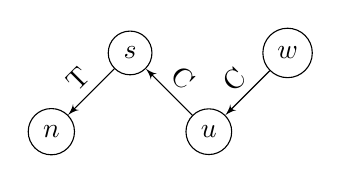
\begin{tikzpicture}
			\tikzset{vertex/.style = {shape=circle,draw,minimum size=1.5em}}
			\tikzset{edge/.style = {->,> = latex'}}
			% vertices
			\node[vertex] (s) at (0, 0) {$s$};
			\node[vertex] (n) at (-1, -1) {$n$};
			\node[vertex] (u) at (1, -1) {$u$};
			\node[vertex] (w) at (2, 0) {$w$};
			% edges
			\draw[edge] (s) -- (n) node[midway, above, rotate=45] {T};
			\draw[edge] (u) -- (s) node[midway, above, rotate=-45] {C};
			\draw[edge] (w) -- (u) node[midway, above, rotate=45] {C};
		\end{tikzpicture}
	\end{figure*}
	\FloatBarrier
	\paragraph{Exercise 12}
	There exists at least one path between every two vertices in a connected component. So if we perform DFS on an arbitrary vertex $u$, it will discover all reachable vertices from $u$. After DFS visit all vertices in $u$'s connected component it terminates. So the number of DFS trees is equal to the number of connect components in undirected graph. This is not true for directed graphs. Consider figure \ref{fig:NonSinglyConnectedGraph}. If we start from $u$ we only have one DFS tree. But if we start from $v$, $x_1$, $x_2$, $x_3$, $x_4$ and finally $u$, the number of DFS trees are equal to the number of vertices. In other words, all DFS trees are consist of only a vertex and we don't have any tree edges.
	
	\begin{algorithm}[h!]
		\caption{Connected components in an undirected graph}
		\begin{algorithmic}[1]
			\Function{DFS}{G}
				\ForAll{$u \in G.V$}
					\State $u.color = WHITE$
					\State $u.\pi = NIL$
				\EndFor
				\State $time = 0$
				\State $ccn = 0$ \Comment $ccn$ is the number of connected components
				\ForAll{$u \in G.V$}
					\If{u.color == WHITE}
						\State $ccn = ccn + 1$					
						\State \Call{DFS-VISIT}{G, u}
					\EndIf
				\EndFor
			\EndFunction
		\end{algorithmic}
		\begin{algorithmic}
			\Statex
		\end{algorithmic}	
		\begin{algorithmic}[1]
			\Function {DFS-VISIT}{G, u}
			\State $time = time + 1$
			\State $u.d = time$
			\State $u.cc = ccn$
			\State $u.color = GRAY$
			\ForAll{$v \in G.adj[u]$}
			\If{$v.color == WHITE$}
			\State $v.\pi = u$
			\State \Call{DFS-VISIT}{$G, v$}
			\EndIf
			\EndFor
			\State $u.color = BLACK$
			\State $time = time + 1$
			\State $u.f = time$
			\EndFunction			
		\end{algorithmic}
	\end{algorithm}
	\FloatBarrier
	\paragraph{Exercise 13}
	It is obvious that we should only have tree and back edges and possibly some cross edges. If we have a cross edge in the same DFS tree it's not a singly connected graph. But If we have cross edges between different DFS trees, it's possible that it's not a single connected graph (See figure \ref{fig:GraphOfComponents}). It is important to start from the right vertex. Consider figure \ref{fig:NonSinglyConnectedGraph}. There is exactly two distinct paths between $u$ and $v$. If we start the DFS from $u$, in the first run we can detect that the graph is not singly connected.
	\begin{figure}[h!]
		\centering
		\caption{non singly connected graph}
		\label{fig:NonSinglyConnectedGraph}		
		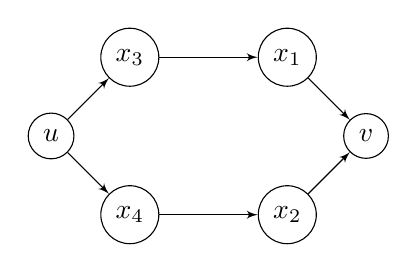
\begin{tikzpicture}
		\tikzset{vertex/.style={shape = circle, draw, minimum size = 1.5em}}
		\tikzset{edge/.style={->, > = latex'}}
		\tikzset{snake it/.style={-stealth,
				decoration={snake, 
					amplitude = 1mm,
					segment length = 8mm,
					post length=0.9mm},decorate}}
		%vertices
		\node[vertex] (u) at (0, 0) {$u$};
		\node[vertex] (x3) at (1, 1) {$x_3$};
		\node[vertex] (x4) at (1, -1) {$x_4$};
		\node[vertex] (x1) at (3, 1) {$x_1$};
		\node[vertex] (x2) at (3, -1) {$x_2$};
		\node[vertex] (v) at (4, 0) {$v$};
		%edges
		\draw[edge] (u) -- (x3);
		\draw[edge] (u) -- (x4);
		\draw[edge] (x3) -- (x1);
		\draw[edge] (x4) -- (x2);
		\draw[edge] (x1) -- (v);
		\draw[edge] (x2) -- (v);
		\end{tikzpicture}
	\end{figure}
	I thought I can design an $O(V + E)$ algorithm to solve this problem. I was wrong.
	\subparagraph{Wrong idea 1}
	Start DFS from an arbitrary vertex $s$. If you found "forward" or "cross" edges then it is not singly connected so the algorithm terminates. After DFS finished, it is possible we have unvisited vertices.
	
	\subparagraph{Wrong idea 2}
	\begin{itemize}
		\item[] \textbf{component:} All undiscovered vertices which will be discover in one DFS run. For example if we run DFS from $x_3$ in figure \ref{fig:NonSinglyConnectedGraph}, $x_3$, $x_1$ and $u$ are belong to the same component. In other words a component is a DFS tree
	\end{itemize}
	We can determine and number the components (similar to connected components). If we find "forward" or "cross" edges within each component, the algorithm terminates. Note that "cross" edges between components is not trivial. We can have singly connected graph which has at least one cross edge between its components. We can create a new graph which its vertices are the components of input graph and its edges are the cross edges between components. Suppose in figure \ref{fig:NonSinglyConnectedGraph} we run DFS first on $x_3$, then $x_4$ and finally $u$. You can see the result in figure \ref{fig:GraphOfComponents}. This algorithm is not always correct. Suppose we run DFS again on new graph (figure \ref{fig:GraphOfComponents}) first on node $\{x_3, x_1, v\}$, then $\{x_4, x_2\}$ and finally $\{u\}$. As you can see we don't have any tree edges but only cross edges. In this scenario we cannot combine some nodes to get a new graph with smaller number of nodes.
	\begin{figure}[h!]
		\centering
		\caption{Graph of components}
		\label{fig:GraphOfComponents}
		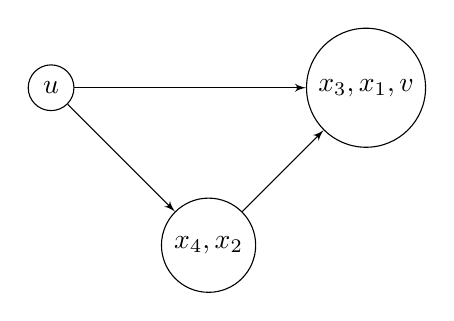
\begin{tikzpicture}
		\tikzset{vertex/.style={shape = circle, draw, minimum size = 1.5em}}
		\tikzset{edge/.style={->, > = latex'}}
		\tikzset{snake it/.style={-stealth,
				decoration={snake, 
					amplitude = 1mm,
					segment length = 8mm,
					post length=0.9mm},decorate}}
		%vertices
		\node[vertex] (u) at (0, 0) {$u$};
		\node[vertex] (x4) at (2, -2) {$x_4, x_2$};
		\node[vertex] (v) at (4, 0) {$x_3, x_1, v$};
		%edges
		\draw[edge] (u) -- (v);
		\draw[edge] (u) -- (x4);
		\draw[edge] (x4) -- (v);
		\end{tikzpicture}
	\end{figure}
	\subparagraph{Wrong Idea 3}
	If you google for solution you may find a solution which suggest to run topological sort. This algorithm assumes that we have at least one vertex with indegree zero which is not a correct assumption for singly connected graph.
	\subparagraph{Correct Answer}
	Since we don't know on which vertex we must start the DFS algorithm, we run DFS on every vertex $v \in V$. In every run we initialize all vertices attributes (.e.g $v.color = WHITE$). If we encounter forward or cross edges (note that we reset attributes in each run, so the cross edges are only in the same DFS tree and we don't encounter cross edges between two different DFS trees), we know that it's not singly connected. In each iteration we visit vertices at most $|E| + 1$ times. so the total runtime of this algorithm is $O(V \times (E + 1)) = O(V + VE)$.
	
	\section{Topological Sort}
	\paragraph{Exercise 2}
	Note that since it's a acyclic graph, we cannot have back edges. We add an attribute name $path$ to each vertex which holds the number of simple paths from that vertex to $t$. The running time of this algorithm is $O(V + E)$.
	\begin{algorithm*}
		\begin{algorithmic}[1]
			\Function {DFS}{G, s, t}
				\ForAll{$u \in G.V$}
					\State $u.color = WHITE$
					\State $u.\pi = NIL$
					\State $u.path = 0$	\Comment $u.path$ is the number of simple paths from $u$ to $t$
				\EndFor
			\State $time = 0$
			\State \Call{DFS-VISIT}{$G, s, t$}
			\EndFunction
			
			\Function {DFS-VISIT}{G, u, t}	
				\State $time = time + 1$
				\State $u.d = time$
				\State $u.color = GRAY$
				\If{$u == t$}
					\State $u.path = 1$
					\State $u.color = BLACK$
					\State return
				\EndIf
				\ForAll{$v \in G.adj[u]$}
					\If{$v.color == WHITE$} \Comment edge $(u, v)$ is a tree edge
						\State $v.\pi = u$
						\State \Call{DFS-VISIT}{$G, v, t$}
						\State $u.path = u.path + v.path$					
					\ElsIf{$u.d < v.d$}	\Comment edge $(u, v)$ is a forward edge
						\State $u.path = u.path + v.path$
					\Else	\Comment edge $(u, v)$ is a cross edge
						\State $u.path = u.path + v.path$
					\EndIf
				\EndFor
				\State $u.color = BLACK$
				\State $time = time + 1$
				\State $u.f = time$
			\EndFunction
		\end{algorithmic}
	\end{algorithm*}
	\FloatBarrier	
	\paragraph{Exercise 3}
	Since the graph is undirected, we encounter only tree and back edges. Note that for all tree edges $(u, v)$, edge $(v, u)$ is a back edge. In this case we consider it as tree edge. In other words, we assume that if edge $(u, v)$ is a back edge, then $v$ is not the parent of $u$. We start DFS on the graph If we encounter a back edge, we terminate the algorithm immediately. We visit every vertex only once. We also visit tree edges only once. If the DFS tree has at least one back edge, we only visit one of those back edges. So the running time of algorithm is the number of vertices plus the number of tree edges plus one back edge: $O(V + V - 1 + 1) = O(V)$.
	
	\begin{algorithm*}
		\begin{algorithmic}[1]
			\Function {DFS-VISIT}{G, u}
				\State $time = time + 1$
				\State $u.d = time$
				\State $u.color = GRAY$
				\ForAll{$v \in G.adj[u]$}
					\If{$v.color == WHITE$} \Comment tree edge
						\State $v.\pi = u$
						\If {\Call{DFS-VISIT}{$G, v$}}
							\State return TRUE
						\EndIf
					\ElsIf{$v.color == GRAY \land v.\pi == u$} \Comment  tree edge
						\State continue
					\ElsIf{$v.color == GRAY \land v.\pi \ne u$} \Comment back edge
					\State return TRUE
					\Else	\Comment $v.COLOR$ is BLACK
						\State continue	\Comment we never reach this
					\EndIf
				\EndFor
				\State $u.color = BLACK$
				\State $time = time + 1$
				\State $u.f = time$
				\State return FALSE
			\EndFunction
		\end{algorithmic}
	\end{algorithm*}
	\FloatBarrier
	
	\section{Strongly connected components}
	The algorithm for SCC:
	
	\begin{enumerate}
	\item call $DFS(G)$ to compute finishing time $u.f$ for all vertices $u \in G.V$
	\item Compute $G^T$. Remember $(u, v) \in G^T.V$ if $(v, u) \in G.V$
	\item call $DFS(G^T)$, but in the main loop of $DFS$ (the loop in which you run DFS-VISIT for white vertices), consider the vertices in order of decreasing $u.f$ (as computed in line 1). In other words run $DFS(G^T)$ in topological sort order of $DFS(G)$ which is computed in line 1
	\item output the vertices of each tree in the depth-first forest formed in line 3 as a separate strongly connected component. We are, in essence, visiting the vertices of the component graph (each of which corresponding to a strongly connected component of G) in topologically sorted order.
	\end{enumerate}
	
	To understand the algorithm consider following paragraphs from textbook:
	
	\paragraph{Lemma 22.13} Let $C$ and $C^\prime$ be distinct strongly connected components in directed graph $G = (V, E)$, let $u, v \in C$, let $u^\prime, v^\prime \in C^\prime$, and suppose that $G$ contains a path $u \rightsquigarrow u^\prime$. Then $G$ cannot also contain a path $v^\prime \rightsquigarrow v$.
	
	\paragraph{Definitions}If $U \subseteq V$, then we define $d(U)=\min_{u \in U}\{u.d\}$ and $f(U) = \max_{u \in U}\{u.f\}$. That is, $d(U)$ and $f(U)$ are the earliest discovery time and latest finishing time, respectively, of any vertex in $U$.
	
	\paragraph{Lemma 22.14} Let $C$ and $C^\prime$ be distinct strongly connected components in directed graph $G=(V,E)$. Suppose that there is an edge $(u, v) \in E$, where $u \in C$ and $v \in C^\prime$. Then $f(C) > f(C^\prime)$.
	
	\paragraph{Corollary 22.15} Let $C$ and $C^\prime$ be distinct strongly connected components in directed graph $G=(V,E)$. Suppose that there is an edge $(u, v) \in E^T$, where $u \in C$ and $v \in C^\prime$. Then $f(C) < f(C^\prime)$. In other words each edge in $G^T$ that goes between different strongly connected components goes from a component with an earlier finishing time (in the first-depth search) to a component with a later finishing time.
	
	\paragraph{Understanding strongly connected component algorithm} Let us examine what happens when we perform the second DFS, which is on $G^T$. We start with strongly connected component $C$ whose finishing time $f(C)$ is maximum. The search starts from some vertex $x \in C$, and it visits all vertices in $C$. By Corollary 22.15, $G^T$ contains no edge from $C$ to any other strongly connected component, and so the search from $x$ will not visit vertices in any other component. Thus, the tree rooted at $x$ contains exactly the vertices of $C$. Having completed visiting all vertices in $C$, the search in line 3 (SCC algorithm) selects as a root a vertex from some other strongly connect component $C^\prime$ whose finishing time $f(C^\prime)$ is maximum over all components other than $C$. Again, the search will visit all vertices in $C^\prime$, but by Corollary 22.15, the only edges in $G^T$ from $C^\prime$ to any other component must be to $C$, which we have already visited. In general, when the DFS of $G^T$ in line 3 visits any strongly connected component, any edges out of that component must be to components that the search already visited.Each depth-first tree, therefore, will be exactly one strongly connected component.
	
	\paragraph{Tricky point} You may think that we can run the second DFS on $G$ instead of $G^T$ and we need to sort vertices in decreasing order of their finishing time. It's not always correct. See exercise 3.
	
	\paragraph{Exercise 3}
	Not always. See the following graph. Suppose in the first DFS we start from $s$, then visit $u$ and finally we visit $v$. In other words, $s.d < u.d < u.f < v.d < v.f < s.f$. So in the second DFS, we start from $u$ and both $s$ and $v$ are reachable from $u$. It means that all $u$ and $s$ and $v$ are in the same component which is wrong.
	
	\begin{figure*}[h!]
		\centering
		\caption{Counterexample}
		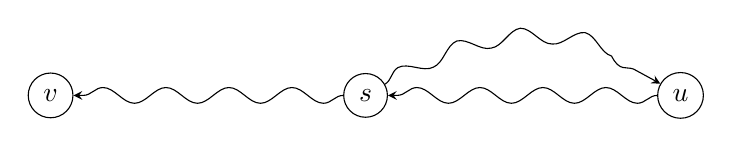
\begin{tikzpicture}
		\tikzset{vertex/.style={shape = circle, draw, minimum size = 1.5em}}
		\tikzset{edge/.style={->, > = latex'}}
		\tikzset{snake it/.style={-stealth,
				decoration={snake, 
					amplitude = 1mm,
					segment length = 8mm,
					post length=0.9mm},decorate}}			
					%vertices
					\node[vertex] (s) at (4, 0) {$s$};
					\node[vertex] (u) at (8, 0) {$u$};
					\node[vertex] (v) at (0, 0) {$v$};
					%edges
					\path[edge] (s) edge[snake it, bend left] (u);
					\path[edge] (u) edge[snake it] (s);
					\path[edge] (s) edge[snake it] (v);
					
					\end{tikzpicture}
					\end{figure*}	
	
	\FloatBarrier
	
	Note in SCC algorithm we say $f(C) > f(C^\prime)$ if there is an edge $(u, v)$ in which $u \in C \land v \in C^\prime$. $f(C)$ means $max_{u \in C}{\{f_u\}}$. Let say $C$ has a vertex $x$ in which its $f_x$ is minimum among all the vertices in Graph. It doesn't guarantee that $f(C)$ is maximum among all SCCs. Because it's possible that $C$ is discovered before $C^\prime$ so there is a vertex $x \in C$ that $f_x \le f_y$ in which $y \in C \cup C\prime$. So if we run DFS on $x$ for sure we will visit all vertices in $C^\prime$ so we consider both $C$ and $C\prime$ as one SCC which is wrong. On the other hand, if we first discover $C^\prime$ then this algorithm works correctly.
	
	\paragraph{Exercise 7}
	
	\subparagraph{Wrong idea} Convert the directed graph to an undirected graph and then run a DFS to see if all vertices are reachable from the root of DFS tree. This algorithm doesn't work. This algorithm consider the following graph as a semiconnected graph which is wrong:	
	
	\begin{figure*}[h!]
		\centering
		\caption{Counterexample}
		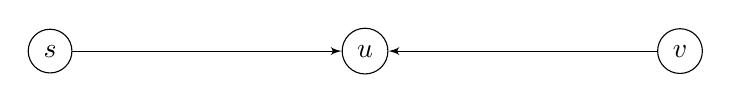
\begin{tikzpicture}
		\tikzset{vertex/.style={shape = circle, draw, minimum size = 1.5em}}
		\tikzset{edge/.style={->, > = latex'}}
		\tikzset{snake it/.style={-stealth,
				decoration={snake, 
					amplitude = 1mm,
					segment length = 8mm,
					post length=0.9mm},decorate}}			
					%vertices
					\node[vertex] (s) at (0, 0) {$s$};
					\node[vertex] (u) at (4, 0) {$u$};
					\node[vertex] (v) at (8, 0) {$v$};
					%edges
					\draw[edge] (s) -- (u);
					\draw[edge] (v) -- (u);
					
					\end{tikzpicture}
					\end{figure*}	
	
	\FloatBarrier
	
	\subparagraph{Answer}
	\begin{enumerate}
	\item Call strongly connected components algorithm on $G$.
	\item Form the component graph (each vertex represent a strongly connected component and each edge connect two different strongly connected components).
	\item Since component graph is a directed acyclic graph, you can run topological sort on it. Suppose we stored the sorted vertices in the $L = \{v_1, v_2, \dots, v_n\}$.
	\item Verify there are edges $(v_i, v_{i+1})$ for $i = 1$ to $i = n - 1$.
	\end{enumerate}
	
	\chapter{Minimum Spanning Trees}
	For questions similar to Prim's minimum spanning tree see "Variants" in chapter \ref{psec:ShortestPathClassification}.
	\section{The algorithms of Kruskal and Prim}
	Suppose $L = \{(u_1, v_1), (u_2, v_2), \dots, (u_{|E|}, v_{|E|})\}$ such that $(u_i, v_i) \in E \land (u_{i + 1}, v_{i + 1}) \in E \land w(u_i, v_i) \le w(u_{i + 1}, v_{i + 1})$ for all $1 \le i \le |E| - 1$.
	
	\begin{algorithm}[h!]
		\caption{MST-Kruskal. Depending on data structure can be $O(E\log{V})$}
		\begin{algorithmic}
			\Function{MST-PRIM}{$G,w$}
			\State $A = \emptyset$
			\ForAll{$v \in G.V$}
				\State \Call{Make-Set}{$v$}
			\EndFor
			\State L = \Call{Create-List-L}{$G, w$} \Comment $O(E\log{E}) = O(E\log{V^2}) = O(E\log{V})$
			\ForAll{$(u, v) \in L$}
				\If{\Call{Find-Set}{u} $\ne$ \Call{Find-Set}{v}}
					\State $A = A \cup \{(u, v)\}$
					\State \Call{Union}{$u, v$}
				\EndIf
			\EndFor
			\EndFunction
		\end{algorithmic}
	\end{algorithm}
	
		\begin{algorithm}[h!]
			\caption{MST-Prim. $O(V\log{V} + E\log{V}) = O(E\log{V})$}
			\begin{algorithmic}
				\Function{MST-PRIM}{$G,w,r$}
					\ForAll{$u \in G.V$}
						\State $u.key = \infty$
						\State $u.\pi = NIL$
					\EndFor
					\State $r.key = 0$
					\State $Q = G.V$
					\While{$Q \ne \emptyset$}
						\State $u =$\Call{Extract-Min}{Q} \Comment $O(V\log{V})$
						\ForAll{$v \in G.adj[u]$} \Comment $O(E\log{V})$
							\If{$v \in Q \land w(u, v) < v.key$}
								\State $v.\pi = u$
								\State $v.key = w(u, v)$
							\EndIf
						\EndFor
					\EndWhile
				\EndFunction
			\end{algorithmic}
		\end{algorithm}
		\FloatBarrier	
	
	For a simple $O(V^2)$ implementation of Prim algorithm see exercise 2.
	\paragraph{Exercise 2}
	We add a new variable named $u.MST$ to every vertex of graph. It's a boolean variable. It determines whether or not the vertex belongs to minimum spanning tree. As you can see I didn't use an adjacency matrix. You can easily replace it with adjacency matrix. The running time of this algorithm is $O(V^2)$. To be more specific, finding the minimum safe edge (lines 10-15) takes $O(V^2)$. Updating the keys (lines 17-22) takes no more than the sum of out-degree of each vertex. As we know 
	\begin{equation*}
		\sum_{u = \in V} {indegree(u) + outdegree(v)} = 2 \times |E| \le 2 \times |V|^2
	\end{equation*}
	So the total running time of this algorithm is $O(V^2 + 2 \times V^2) = O(V^2)$.
	
	\begin{algorithm}[h!]
		\caption{MST-Prim in $O(V^2)$}
		\begin{algorithmic}[1]
			\Function{MST-PRIM}{$G,w,r$}
				\ForAll{$u \in G.V$}
					\State $u.key = \infty$
					\State $u.\pi = NIL$
					\State $u.MST = FALSE$
				\EndFor
				\State $r.key = 0$
				\For {$c = 1$ TO $c = |G.V|$}
					\State $min = \infty$
					\ForAll{$w \in G.V$}
						\If{$w.MST == FALSE \land w.key < min$}
							\State $min = w.key$
							\State $u = w$
						\EndIf
					\EndFor
					\State $u.MST = TRUE$
					\ForAll{$v \in G.adj[u]$}
						\If{$v.MST == FALSE \land w(u, v) < v.key$}
							\State $v.\pi = u$
							\State $v.key = w(u, v)$
						\EndIf
					\EndFor
				\EndFor
			\EndFunction
		\end{algorithmic}
	\end{algorithm}
	\FloatBarrier	
	\section{Problems}
	\paragraph{Problem 3 Bottleneck spanning tree}
	\subparagraph{a.}
	Consider an arbitrary MST $T$. Suppose the maximum-weight edge in $T$ is $e$. If we remove that edge we have a forest of two trees $C_1$ and $C_2$. Now consider MST $T'$ whose maximum-weight edge, $e'$, is less that $e$. There should be an edge in $T'$ that connects $C_1$ to $C_2$. The weight of that edge should be less than $e$. In other words, $e$ is not a light edge which contradicts $T$ is an MST.
	\subparagraph{b.}
	We remove all edges in $G.E$ which their weight are higher than $b$. We called the modified graph $G_b$. It is obvious that $G_b.V = G.V$ and $G_b.E = \{(u, v) \in G.E : w(u, v) \le b\}$. If $G_b$ remains connected then every spanning tree of $G_b$ doesn't have an edge whose weight is greater than b. The running time of this algorithm is $O(V + E)$. Since G should be a connected graph, $|E| \ge |V| - 1$. So we can say the running time is $O(E)$.
	\begin{algorithm*}[h!]
		\begin{algorithmic}[1]
			\Function{VALID-BST-VALUE}{G, b}
				\State $G' = $ \Call{REMOVE-EDGES}{G, b}
				\State \Call{InitDFS}{$G'$}
				\State $c = 0$ \Comment The number of connected components
				\ForAll{$u \in G'.V$}
					\If{$u.color == WHITE$}
						\State $c = c + 1$
						\State \Call{DFS}{$G'$, u}
					\EndIf
				\EndFor
				\State \Return $(c == 1)$
			\EndFunction
		\end{algorithmic}
	\end{algorithm*}
	\begin{algorithm*}[h!]
		\begin{algorithmic}[1]
			\Function{REMOVE-EDGES}{G, b}
				\State $G_b.V = G.V$
				\State $G_b.E = \emptyset$
				\ForAll{$(u, v) \in G.E$}
					\If{$(u, v).c \le b$} \Comment $(u, v).c \equiv w(u, v)$
						\State $G_b.E = G_b.E \cup \{(u, v)\}$
					\EndIf					
				\EndFor
				\State \Return $G_b$
			\EndFunction
		\end{algorithmic}
	\end{algorithm*}		
	\FloatBarrier
	\subparagraph{c.}
	We need some definitions:
	\begin{itemize}
		\item $\boldsymbol{G_b:}$ a new sub-graph of $G$ which $G_b.V = G.V$ and $G_b.E = \{(u, v) \in G.E : w(u, v) \le b\}$
		\item $\boldsymbol{comp(u):}$ Suppose connected components $c_1, c_2, \dots, c_k$ make the Graph $G_b$ and vertex $u$ belongs to the i\textsuperscript{th} component. Then $comp(u) = i$
		\item $\boldsymbol{G'_b:}$ Suppose $C = \{c_1, c_2, \dots, c_k\}$ is the set of connected components of $G_b$. Then $G'_b.V = C$ and $G'_b.E = \{(u, v) \in G.E : comp(u) \ne comp(v)\}$. It is possible that there are more than one edge between $c_i$ and $c_j$. In this case we choose the light edge (minimum weight)
	\end{itemize}
	We want to find $b_{m} = \min\limits_{b \in G.E \land |G'_b.V| = 1}(b)$. In other words, we want to find the minimum of $b \in G.E$ which $G_b$ is a connected graph. Consider an arbitrary edge $(u, v)$. Suppose $w(u, v) = b$ There are two cases:
	\begin{enumerate}
		\item $\boldsymbol{G_b}$\textbf{ is connected:} It means $b_m < b$. More precisely, $b_m \in G_b.E$
		\item $\boldsymbol{G_b}$\textbf{ is not connected:} It means $b_m \ge b$. More precisely, $b_m \in G'_b.E$. 
	\end{enumerate}
	Consider set $W = {w(u, v) : (u, v) \in G.E}$. We can find the median of $W$ in $O(E)$ by "median of medians" algorithm. After finding the median, we can divide the edges into two equal sets: $G_b.E$ and $G'_b.E$. In each step we eliminate half of edges. For simplicity we assume edge $(u, v)$ has an attribute $c$ such that $(u, v).c = w(u, v)$.
	\begin{algorithm*}[h!]
		\begin{algorithmic}[1]
			\Function{BST}{G}
				\If{$|G.E| == 1$}
					\State \Return $G.E$
				\EndIf
				\State $m = $ \Call{FIND-MEDIAN}{$G.E$} \Comment $O(E)$
				\If{\Call{VALID-BST-VALUE}{G, m}}
					\State $G_b = $ \Call{REMOVE-EDGES}{G, m} \Comment $O(E)$
					\State $R = $ \Call{BST}{$G_b$}
				\Else
					\State $G'_b = $ \Call{MAKE-$G'_b$}{G} \Comment $O(E)$
					\State $R = $ \Call{BST}{$G'_b$}
				\EndIf
				\State \Return $R$
			\EndFunction
		\end{algorithmic}
	\end{algorithm*}
	
	\begin{algorithm*}[h!]
		\begin{algorithmic}[1]
			\Function{MAKE-$G'_b$}{G}
				\State C, comp = \Call{CC}{G}
				\State $G'_b.V = C$
				\ForAll{$(u, v) \in G.E$}
					\If{$comp[u] \ne comp[v]$}
						\If{$(comp[u], comp[v]) \not\in G'_b.E$}
							\State $(comp[u], comp[v]).c = (u, v).c$
							\State $G'_b.E = G'_b.E \cup \{(comp[u], comp[v])\}$
						\ElsIf{$(u, v).c < (comp[u], comp[v]).c$}
							\State $(comp[u], comp[v]).c = (u, v).c$
						\EndIf
					\EndIf
				\EndFor
				\State \Return $G'_b$
			\EndFunction
		\end{algorithmic}
	\end{algorithm*}
	
	\begin{algorithm*}[h!]
		\begin{algorithmic}[1]
			\Function{CC}{G}
				\State Let $comp[1..G.V]$ be a new array
				\State $C = \emptyset$ \Comment The set of connected components
				\State $c = 0$ \Comment The number of connected components
				\State \Call{INIT-DFS}{G}
				\ForAll{$u \in G.V$}
					\If{$u.color == WHITE$}
						\State $c = c + 1$
						\State $C = C \cup \{c\}$
						\State \Call{DFS}{G, u, c, comp}
					\EndIf
				\EndFor
				\State \Return $C, comp$
			\EndFunction
		\end{algorithmic}
	\end{algorithm*}
	
	\begin{algorithm*}[h!]
		\begin{algorithmic}[1]
			\Function{DFS}{G, u, c, comp}
				\State $u.color = GRAY$
				\State $comp[u] = c$
				\ForAll{$v \in G.adj[u]$}
					\If{$v.color == WHITE$}
						\State \Call{DFS}{G, v, c, comp}
					\EndIf
				\EndFor
			\EndFunction
		\end{algorithmic}
	\end{algorithm*}
	So the total running time of algorithm is $O(E)$:
	\begin{equation*}
		\begin{split}
		T(E) &= T(\frac{E}{2}) + O(E) \\
		&= O(E) + O(\frac{E}{2}) + O(\frac{E}{4}) + \dots + O(\frac{E}{2^i}) + \dots + O(1) \\
		&= O(\frac{E}{2^0}) + O(\frac{E}{2^1}) + \dots + O(\frac{E}{2^{log_2{E}}}) \\
		&= \frac{E(\frac{1}{2})^{log_2{E} + 1} - E}{\frac{1}{2} - 1} \\
		&= 2E - 1
		\end{split}
	\end{equation*}
	For the analysis of run-time we assumed $G$ is connected so $|E| \ge |V| - 1$.
	\chapter{Single-Source Shortest Path}
	
	For the following algorithms we are using these functions:
		\begin{algorithm}[h!]
			\begin{algorithmic}[1]
				\Function{Initialize-Single-Source}{$G,s$}
					\ForAll{$v \in G.V$}
						\State $v.d = \infty$
						\State $v.\pi = NIL$
					\EndFor
					\State s.d = 0
				\EndFunction
			\end{algorithmic}
			
			\begin{algorithmic}[1]
				\Function{Relax}{$u, v, w$}
					\State relaxed = FALSE
					\If{$v.d > u.d + w(u, v)$}
						\State $v.d = u.d + w(u, v)$
						\State $v.\pi = u$
						\State relaxed = TRUE
					\EndIf
					\State return relaxed
				\EndFunction
			\end{algorithmic}			
		\end{algorithm}		
	
	\section{The Bellman-Ford algorithm}		
		\begin{algorithm}[h!]
			\caption{Bellman-Ford algorithm which runs in $O(VE)$}
			\begin{algorithmic}[1]
				\Function{Bellman-Ford}{$G,w,s$}
					\State \Call{Initialize-Single-Source}{G,s}
					\For{$i = 1$ TO $|G.V| - 1$}
						\State relaxed = FALSE
						\ForAll{$(u, v) \in G.E$}
							\State relaxed = \Call{Relax}{u, v, w} $\lor$ relaxed
						\EndFor
						\If{$relaxed == FALSE$}
							\State break
						\EndIf
					\EndFor
					\ForAll{$(u, v) \in G.E$}
						\If{$v.d > u.d + w(u, v)$}
							\State return FALSE
						\EndIf
					\EndFor
					\State return TRUE
				\EndFunction
			\end{algorithmic}
		\end{algorithm}
		\FloatBarrier	
	\subsection{Exercises}
	\paragraph{Exercise 3}
	Since finding all shortest-paths require at most $m$ steps, it is obvious in $(m + 1)$\textsuperscript{th} iteration no $u.d$ will be updated for all $u \in V$.
	\begin{algorithm*}[h!]
		\begin{algorithmic}[1]
			\Function{BELLMAN-FORD2}{G, w, s}
				\State \Call{INITIALIZE-SINGLE-SOURCE}{G, s}
				\For{$i = 1$ \textbf{ to } $|G.V| - 1$}
					\State $updated = FALSE$
					\ForAll{edge $(u, v) \in G.E$}
						\If{\Call{RELAX}{u, v, w} $ == TRUE$}
							\State $updated = TRUE$
						\EndIf
					\EndFor
					\If{updated $ == FALSE$}
						\State break
					\EndIf
				\EndFor
			\EndFunction
		\end{algorithmic}
	\end{algorithm*}
	\begin{algorithm*}[h!]
		\begin{algorithmic}
			\Function{RELAX}{u, v, w}
				\If{$v.d > u.d + w(u, v)$}
					\State $v.d = u.d + w(u, v)$
					\State $v.\pi = u$
					\State \Return $TRUE$
				\Else
					\State \Return $FALSE$
				\EndIf
			\EndFunction
		\end{algorithmic}
	\end{algorithm*}
	\FloatBarrier
	\paragraph{Exercise 4}
	When we detect a negative cycle, we need to update $u.d = -\infty$. Then we need to update $d$ attribute for all reachable vertices from $u$ to $-\infty$.
	\begin{algorithm*}[h!]
		\begin{algorithmic}[1]
			\Function{BELLMAN-FORD-MODIFIED}{G, w, s}
				\State \Call{INITIALIZE-SINGLE-SOURCE}{G, s}
				\For{$i = 1$ \textbf{ to } $|G.V| - 1$}
					\ForAll{edge $(u, v) \in G.E$}
						\State \Call{RELAX}{u, v, w}
					\EndFor
				\EndFor
				\State \Call{INITIALIZE-DFS}{G}
				\For{each edge $(u, v) \in G.E$}
					\If{$v.d > u.d + w(u, v)$}
						\State $v.d = -\infty$
						\State \Call{DFS}{G, v}
					\EndIf
				\EndFor
			\EndFunction
		\end{algorithmic}
	\end{algorithm*}
	\begin{algorithm*}[h!]
		\begin{algorithmic}[1]
			\Function{DFS}{G, u}
				\State $u.color = GREY$
				\ForAll{$v \in G.adj[u]$}
					\If{$v.color == WHITE$}
						\State $v.d = -\infty$
						\State $v.color = GREY$
						\State \Call{DFS}{G, v}
					\EndIf
				\EndFor
			\EndFunction
		\end{algorithmic}
	\end{algorithm*}
	\FloatBarrier
	\paragraph{Exercise 5}
	We need to modify $Relax$ function (note that we can have edges with negative weights):
	\begin{algorithm*}[h!]
		\begin{algorithmic}[1]
			\Function{Relax}{G, w, u, v}
				\If{$v.d > \min(w(u, v), u.d + w(u, v))$}
					\State $v.d = \min(w(u, v), u.d + w(u, v))$
					\State $v.\pi = u$
				\EndIf
			\EndFunction
		\end{algorithmic}

		\begin{algorithmic}[1]
			\Function{Bellman-Ford}{$G,w,s$}
				\State \Call{Initialize-Single-Source}{G,s}
				\For{$i = 1$ TO $|G.V| - 1$}
					\State relaxed = FALSE
					\ForAll{$(u, v) \in G.E$}
						\State relaxed = \Call{Relax}{u, v, w} $\lor$ relaxed
					\EndFor
					\If{$relaxed == FALSE$}
						\State break
					\EndIf
				\EndFor
				\ForAll{$(u, v) \in G.E$}
					\If{$v.d > u.d + w(u, v)$}
						\State return FALSE
					\EndIf
				\EndFor
				\State return TRUE
			\EndFunction
		\end{algorithmic}		
	\end{algorithm*}	
	\FloatBarrier
	\paragraph{Exercise 6}
	We add a new attribute $u.mark$ for avoiding printing vertices in a negative cycle more than once. Suppose $v_0, v_1, \dots, v_k$ are vertices in a negative cycle and $v_0 = v_k$. The Bellman-Ford algorithm expands shortest-path tree in each step. Suppose $v_i.\pi = v_{i - 1}$ for $1 \le i \le k - 1$ and $v_0.\pi = v_k.\pi = u$. Since the cycle is negative, $v_{k - 1}.d + w(k - 1, k) < v_k.d$. So we change the value of $v_k.\pi$ from $u$ to $v_{k - 1}$. In other words, $v_i$ for $0 \le i \le k$ are unreachable from $u$ in shortest-path tree.
	\begin{algorithm*}[h!]
		\begin{algorithmic}[1]
			\Function{BELLMAN-FORD-MODIFIED}{G, w, s}
				\State \Call{INITIALIZE-SINGLE-SOURCE}{G, s}
				\For{$i = 1$ \textbf{ to } $|G.V| - 1$}
					\ForAll{edge $(u, v) \in G.E$}
						\State \Call{RELAX}{u, v, w}
					\EndFor
				\EndFor
				\ForAll{$u \in G.V$}
					\State $u.mark = FALSE$
				\EndFor
				\For{each edge $(u, v) \in G.E$}
					\If{$v.d > u.d + w(u, v)$}
						\State $w = v$
						\While{$w.mark == FALSE$}
							\State $w.mark = TRUE$
							\State \Call{PRINT}{w}
							\State $w = w.\pi$
						\EndWhile
					\EndIf
				\EndFor
			\EndFunction
		\end{algorithmic}
	\end{algorithm*}
	\FloatBarrier	
	\section{Dijkstra's algorithm}
	For an intuition of Dijkstra shortest path, see figure \ref{fig:dijkstra-shortest-path-algorithm}.
	
	
		\begin{algorithm*}[h!]
			\begin{algorithmic}[1]
				\Function{Initialize-Single-Source}{$G,s$}
					\ForAll{$v \in G.V$}
						\State $v.d = \infty$
						\State $v.\pi = NIL$
					\EndFor
					\State s.d = 0
				\EndFunction
			\end{algorithmic}
			
			\begin{algorithmic}[1]
				\Function{Relax}{$u, v, w$}
					\State relaxed = FALSE
					\If{$v.d > u.d + w(u, v)$}
						\State $v.d = u.d + w(u, v)$
						\State $v.\pi = u$
						\State relaxed = TRUE
					\EndIf
					\State return relaxed
				\EndFunction
			\end{algorithmic}
	
			\begin{algorithmic}[1]
				\Function{Dijkstra}{$G,w,s$}
					\State \Call{Initialize-Single-Source}{G,s}
					\State $S = \emptyset$
					\State $Q = G.V$
					\While{$Q \ne \emptyset$}
						\State $u=$ \Call{Extract-Min}{Q}
						\State $S = S \cup \{u\}$
						\ForAll{$v \in G.adv[u]$}
							\State \Call{Relax}{u, v, w}
						\EndFor
					\EndWhile
				\EndFunction
			\end{algorithmic}		
		\end{algorithm*}
		\FloatBarrier
	
	\begin{figure}
	\centering
	\caption{Dijkstra Shortest Path Algorithm}
	\label{fig:dijkstra-shortest-path-algorithm}
	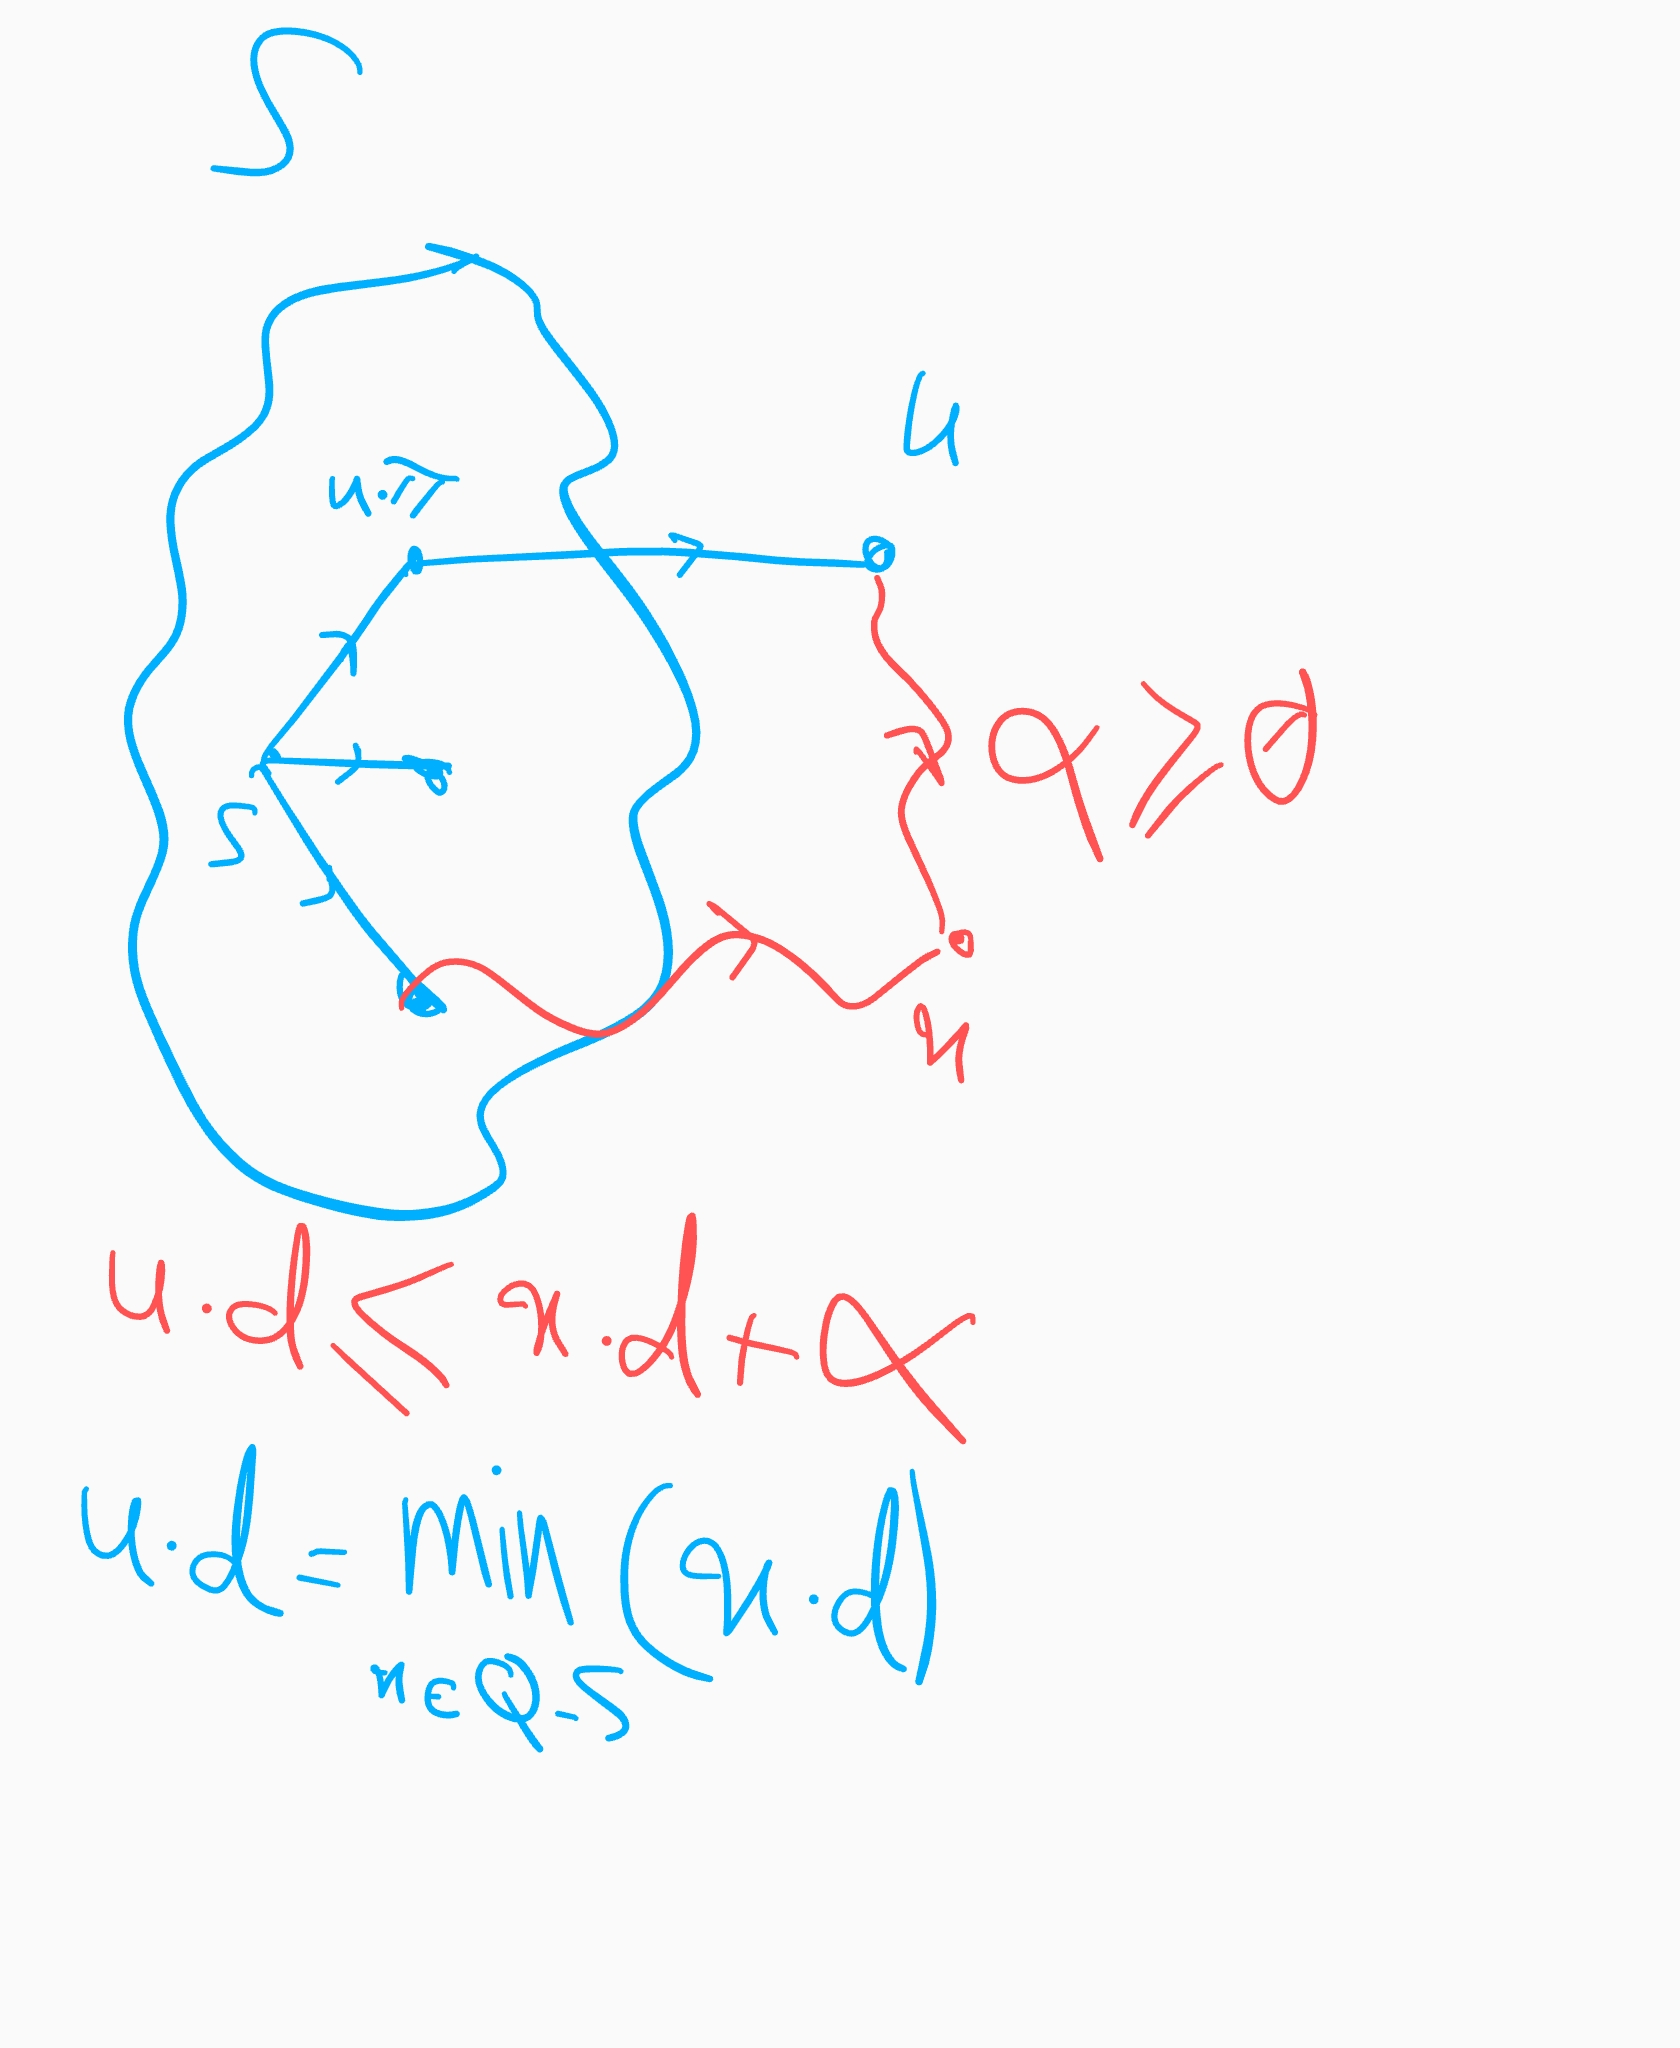
\includegraphics[width=\linewidth]{images/dijkstra-shortest-path.jpg}
	\end{figure}
	\FloatBarrier
	\subsection{Exercises}
	\paragraph{Exercise 6}
	Suppose the path $p = (v_0, v_1, \dots, v_k)$ in which $v_0 = u$ and $v_k = v$ is one of the paths between $u$ and $v$. Since the probabilities are independent we want to find $\max(\prod_{i = 0}^{k - 1}r(v_i, v_{i+1}))$. We can reduce the problem to a shortest-path one by changing the weight function $w(u, v) = r(u, v)$ to $w'(u, v) = -\log{r(u, v)}$.
	\begin{equation*}
	\begin{split}
		0 &\le r(u, v) \le 1 \\
		\log 0 &\le \log{r(u, v)} \le \log 1
	\end{split}
	\end{equation*}
	If we define $\log 0 = -\infty$, then $-\infty \le \log{r(u, v)} \le 0$ which is equivalent to $0 \le -\log{r(u, v)} \le \infty$.
	\begin{equation*}
	\begin{split}
		\max(\prod_{i = 0}^{k - 1}r(v_i, v_{i+1})) \\
		&\equiv \max(\sum_{i = 0}^{k - 1}\log{r(v_i, v_{i+1})}) \\
		&\equiv \min(\sum_{i = 0}^{k - 1}-\log{r(v_i, v_{i+1})})
	\end{split}
	\end{equation*}
	which is exactly the shortest path problem. Since $w'(u, v)$ is non-negative, we can use Dijkstra algorithm which its run-time can be $O(E\log V)$. We only need to change $RELAX$ function.
	\begin{algorithm*}[h!]
		\begin{algorithmic}[1]
			\Function{$w'$}{u, v, w}
				\If{$w(u, v) == 0$}
					\State \Return $\infty$
				\Else
					\State \Return $-\log{w(u, v)}$
				\EndIf
			\EndFunction
		\end{algorithmic}
	\end{algorithm*}
	\begin{algorithm*}
		\begin{algorithmic}[1]
			\Function{RELAX}{u, v, w}
				\If{$v.d > u.d + w'(u, v, w)$}
					\State $v.d = u.d + w'(u, v, w)$
					\State $v.\pi = u$
				\EndIf
			\EndFunction
		\end{algorithmic}
	\end{algorithm*}	
	\FloatBarrier
	
	\phantomsection
	\label{psec:ShortestPathClassification}	
	\paragraph{Variants}
	\begin{enumerate}
	\item \textbf{Single-source shortest-path problem:}
	\begin{enumerate}
		\item Given unweighted undirected graph $G$ and vertices $s$ and $t$. Find the number of shortest path between $s$ and $t$.
		\begin{itemize}
			\item[\textbf{Solution}] For another example about cross edges in BFS see BFS exercise 7 \ref{psec:bfs_exercise_7}. It's similar to all-pair shortest path problem but we solve it through Single-source shortest-path problem. Since the graph is unweighted we use BFS. We define a new attirbute $u.num$ which is the number of shortest path from $s$ to $u$. Because the graph is unweighted we only deal with tree and cross edges (since it's an undirected graph if $(u, v) \in E$, then $(v, u) \in E$; note that if $(u, v)$ is a tree edge, we need to consider $(v, u)$ also as tree edge). It is possible a tree edge be another shortest path which we need to consider it. Suppose edge $(u, v)$ is a cross edge. According to $d$ property (note that $d$ is distance not discovery time) we know that $u.d + 1 \le v.d$ and $v.d + 1 \le u.d$. So we have $-1 \le u.d - v.d \le 1$. So $u.v - v.d$ can have three values -1, 0, 1. Only if $u.d - v.d = 1$ then $u.d + 1$ is another shortest-path for $v$.
			\begin{algorithm*}[h!]
				\begin{algorithmic}[1]
					\Function{FIND-SHORTEST-PATH-COUNT}{G, s, t}
						\State \Call{INIT-BFS}{G}
						\State $s.d = 0$
						\State $s.num = 1$
						\State $s.color = GREY$
						\State $Q = \emptyset$						
						\State \Call{ENQUEUE}{Q, s}
						\While{$Q \ne \emptyset$}
							\State $u = $ \Call{DEQUEUE}{Q}
							\ForAll{$v \in G.adj[u]$}
								\If{$u.color == WHITE$} \Comment $(u, v)$ is a tree edge
									\State $v.color = GREY$
									\State $v.d = u.d + 1$
									\State $v.num = u.num$
									\State \Call{ENQUEUE}{G, v}
								\ElsIf{$u.d + 1 == v.d$}
									\State $v.num = v.num + u.num$
								\EndIf
							\EndFor
						\EndWhile
						\State \Return $t.num$
					\EndFunction
				\end{algorithmic}
			\end{algorithm*}
			\begin{algorithm*}[h!]
				\begin{algorithmic}
					\Function{INIT-BFS}{G}
						\ForAll{$u \in G.V$}
							\State $u.d = \infty$
							\State $u.color = WHITE$
							\State $u.num = 0$
						\EndFor
					\EndFunction
				\end{algorithmic}
			\end{algorithm*}
			\FloatBarrier
		\end{itemize}
		\item Consider two arbitrary vertices $u$ and $v$. Suppose there is path $p$ between $u$ and $v$. We define $m = \min\limits_{(u, v) \in p}(w(u, v))$ and $M = \max\limits_{(u, v) \in p}(w(u, v))$.
		\begin{enumerate}
			\item Find a path between $u$ and $v$ which has the maximum $m$ among all possible paths
			\begin{itemize}
				\item \textbf{Solution} We can use an algorithm similar to Dijkstra's shortest path for solving this problem. Hint: extract the maximum element from $Q$ in each iteration.
			\end{itemize}
			\item Find a path between $u$ and $v$ which has the minimum $M$ among all possible paths
			\begin{itemize}
				\item \textbf{Solution} We can use an algorithm similar to Dijkstra's shortest path for solving this problem
			\end{itemize}			
			\item Find a path between $u$ and $v$ which has the maximum $M$ among all possible paths
			\begin{itemize}
				\item \textbf{Solution} We can't use an algorithm similar to Dijkstra's shortest path. Instead we use an algorithm similar to Bellman-Ford shortest path. It is possible the path has at least one cycle.
			\end{itemize}
			\item Find a path between $u$ and $v$ which has the minimum $m$ among all possible paths
			\begin{itemize}
				\item \textbf{Solution} We can't use an algorithm similar to Dijkstra's shortest path. Instead we use an algorithm similar to Bellman-Ford shortest path. It is possible the path has at least one cycle.
			\end{itemize}
		\end{enumerate}		
		\item acm-icpc World Finals 2002 question C, Crossing the Desert: You can see the problem statement in \href{http://www.spoj.com/problems/DESERT/}{"DESERT Problem in SPOJ"} and \href{https://uva.onlinejudge.org/index.php?option=com_onlinejudge&Itemid=8&page=show_problem&problem=3452}{"Problem 1011 in UVa"} online judges.\\
		In this problem, you will compute how much food you need to purchase for a trip across the desert on foot.\\
		At your starting location, you can purchase food at the general store and you can collect an unlimited amount of free water. The desert may contain oases at various locations. At each oasis, you can collect as much water as you like and you can store food for later use, but you cannot purchase any additional food. You can also store food for later use at the starting location. You will be given the coordinates of the starting location, all the oases, and your destination in a two-dimensional coordinate system where the unit distance is one mile. \\
		For each mile that you walk, you must consume one unit of food and one unit of water. Assume that these supplies are consumed continuously, so if you walk for a partial mile you will consume partial units of food and water. You are not able to walk at all unless you have supplies of both food and water. You must consume the supplies while you are walking, not while you are resting at an oasis. Of course, there is a limit to the total amount of food and water that you can carry. This limit is expressed as a carrying capacity in total units. At no time can the sum of the food units and the water units that you are carrying exceed this capacity. \\
		You must decide how much food you need to purchase at the starting location in order to make it to the destination. You need not have any food or water left when you arrive at the destination. Since the general store sells food only in whole units and has only one million food units available, the amount of food you should buy will be an integer greater than zero and less than or equal to one million. 
		\paragraph{Input}
		The first line of input in each trial data set contains n ($2 \le n \le 20$), which is the total number of significant locations in the desert, followed by an integer that is your total carrying capacity in units of food and water. The next n lines contain pairs of integers that represent the coordinates of the n significant locations. The first significant location is the starting point, where your food supply must be purchased; the last significant location is the destination; and the intervening significant locations (if any) are oases. You need not visit any oasis unless you find it helpful in reaching your destination, and you need not visit the oases in any particular order. \\
		The input is terminated by a pair of zeroes.
		\paragraph{Output}
		For each trial, print the trial number followed by an integer that represents the number of units of food needed for your journey. Use the format shown in the example. If you cannot make it to the destination under the given conditions, print the trial number followed by the word "Impossible."\\
		Place a blank line after the output of each test case.
		\paragraph{Example}
		\subparagraph{Input} \mbox{}\\
		4 100\\
		10 -20\\
		-10 5\\
		30 15\\
		15 35\\
		2 100\\
		0 0\\
		100 100\\
		0 0
		\subparagraph{Output} \mbox{}\\
		Trial 1: 136 units of food\\
		Trial 2: Impossible\\
		\phantomsection
		\begin{itemize}
			\item[\textbf{Solution:}] First we make question simpler. So we suppose it is impossible to leave food on oases or starting location and possibly return and collect them.\\
            We can model this problem to an undirected graph. The vertices are the starting location, oases and the destination. There is an edge between $u$ and $v$, if the amount of required food and water doesn't exceed $C$.
            \begin{itemize}
                    \item $\boldsymbol{f_{u, v}:}$ The amount of required food from $u$ to $v$
                    \item $\boldsymbol{a_{u, v}:}$ The amount of required water from $u$ to $v$
            \end{itemize}
            We define weight function $w$:
            \begin{equation*}
                    w(u, v) = \begin{cases}
                    f_{u, v} & f_{u, v} + a_{u, v} \le C \\
                    \infty & f_{u, v} + a_{u, v} > C
                    \end{cases}
            \end{equation*}
            Unlike food, we can pick up water in every oases. So we need to order all required food in the starting location. Because we cannot leave food anywhere in the desert, the final path should be simple. Otherwise we have at least one cycle. If we remove that cycle we obtain an equivalent path which required less food. Suppose path $p$ which connects the starting location to the target is an optimal path. We define $a_m = \max\limits_{(u, v) \in p}(a(u, v))$. We called $p$ a valid path if $\sum_{(u, v) \in p}{f(u,v)} + a_m \le C$. The required food for $p$ must be minimum among all valid paths from the starting location to the destination. We can solve this problem with a greedy algorithm similar to Dijkstra's shortest path. $u.d$ is the amount of required food from the starting location to $u$. We define a new attribute $u.a_m$ which we described it before. $s$ is the starting location and $t$ is the target location. The running time of algorithm is like Dijkstra's shortest path which can be $O(E\log V)$.
            \begin{algorithm*}[h!]
                    \begin{algorithmic}[1]
                            \Function{Desert}{G, w, C, s, t}
                                    \State \Call{INITIALIZE-SINGLE-SOURCE}{G, s}
                                    \State $S = \emptyset$
                                    \State $Q = G.V$
                                    \While{$Q \ne \emptyset$}
                                            \State $u = $ \Call{EXTRACT-MIN}{G}
                                            \State $S = S \cup \{u\}$
                                            \ForAll{$v \in G.Adj[u]$}
                                                    \State \Call{RELAX}{u, v, w, C}
                                            \EndFor
                                    \EndWhile
                                    \If{$t.d < \infty$}
                                            \State \Return $t.d$
                                    \Else
                                            \State $"IMPOSSIBLE"$
                                    \EndIf
                            \EndFunction
                    \end{algorithmic}
            \end{algorithm*}
            \begin{algorithm*}[h!]
                    \begin{algorithmic}[1]
                            \Function{RELAX}{u, v, w, C}
                                    \State $m = \max(w(u, v), u.a_m)$
                                    \State $food = u.d + w(u, v)$
                                    \If{$(food + m) \le C \land  food < v.d$}
                                            \State $v.d = food$
                                            \State $v.a_m = m$
                                            \State $v.\pi = u$
                                    \EndIf
                            \EndFunction
                    \end{algorithmic}
            \end{algorithm*}
            \begin{algorithm*}[h!]
                    \begin{algorithmic}
                            \Function{INITIALIZE-SINGLE-SOURCE}{G, s}
                                    \ForAll{$v \in G.V$}
                                            \State $v.d = \infty$
                                            \State $v.\pi = NIL$
                                            \State $v.a_m = -\infty$
                                    \EndFor
                                    \State $s.d = 0$
                            \EndFunction
                    \end{algorithmic}
            \end{algorithm*}
            \FloatBarrier
		\end{itemize}
	\end{enumerate}
	\item \textbf{Single-destination shortest-path problem:}
	\begin{enumerate}
		\item You are given flight schedules between a set of $n$ cities. For each pair of cities $(i, j)$ between which there is a direct flight, you are given the pair $(d_{ij}, a_{ij})$, the departure and arrival time of the flight from city $i$ to city $j$. Assume that there is at most one flight from city $i$ to city $j$ per day. Suppose you start at city $A$ and want to reach city $B$. You have an important meeting in city $B$ that you need to attend, and you need to reach city $B$ latest by time $t$. Give an algorithm that outputs a possible sequence of flights you could take starting from city $A$ as late as possible and reaching city $B$ before time $t$, with at least one hour layover between any two consecutive flights.
		\begin{itemize}
			\item[\textbf{Solution:}] We don't know which flight in $A$ we should choose. We can solve the problem if we consder flights in $B$. Given the graph $G$, we need to change that to graph $G'$ such that $G'.V = G.V$ and $G'.E = \{(u, v) : (v, u) \in V.E\}$. Hence if $(i, j) \in G'.E$, there is a flight from $j$ to $i$ in which the departure time is $d_{ji}$ and arrival time is $a_{ji}$. In $B$ we only need to consider all flights $C = \{(B, u) \in G'.E : a_{uB} \le t\}$ and choose the edge with latest departure time ($\max\limits_{(B, u) \in C}(d_{uB})$). Because if we arrive at $u$, flight $(u, B)$ has the latest departure time and it doesn't make any sense to go from $u$ to $B$ through other intermediate vertices (this description is not entirely correct see figure \ref{fig:latest_departure} for more information). So we add edge $(u, B)$ as an optimal answer between $u$ and $B$ (in $G'$ we should say edge $(B, u)$). This algorithm is similar to Prim's minimum spanning tree. We can call it "Single-destination latest-departure problem". We calculate the best possible sequence of flights from $u$ to $B$. Eventually we calculate an optimal path from $A$ to $B$. By "best" we mean the departure time of the first flight is as late as possible and the arrival time is at most $t$ and there is a layover of at least one hour between two consecutive flights. $u.d$ store the latest possible departure from $u$ to $B$. We add a dummy flight from $B$ to an unknown place with departure $t + 1$ to discard all those flights to $B$ with arrival time greater than $t$. $Q$ contains all those vertices which we don't know yet an optimal flight sequence from them to $B$. On the other hand, $S$ contains all those vertices which we found out an optimal flight sequence from them to $B$.
			\begin{figure}
			\centering
			\caption{Algorithm correctness}
			\label{fig:latest_departure}
			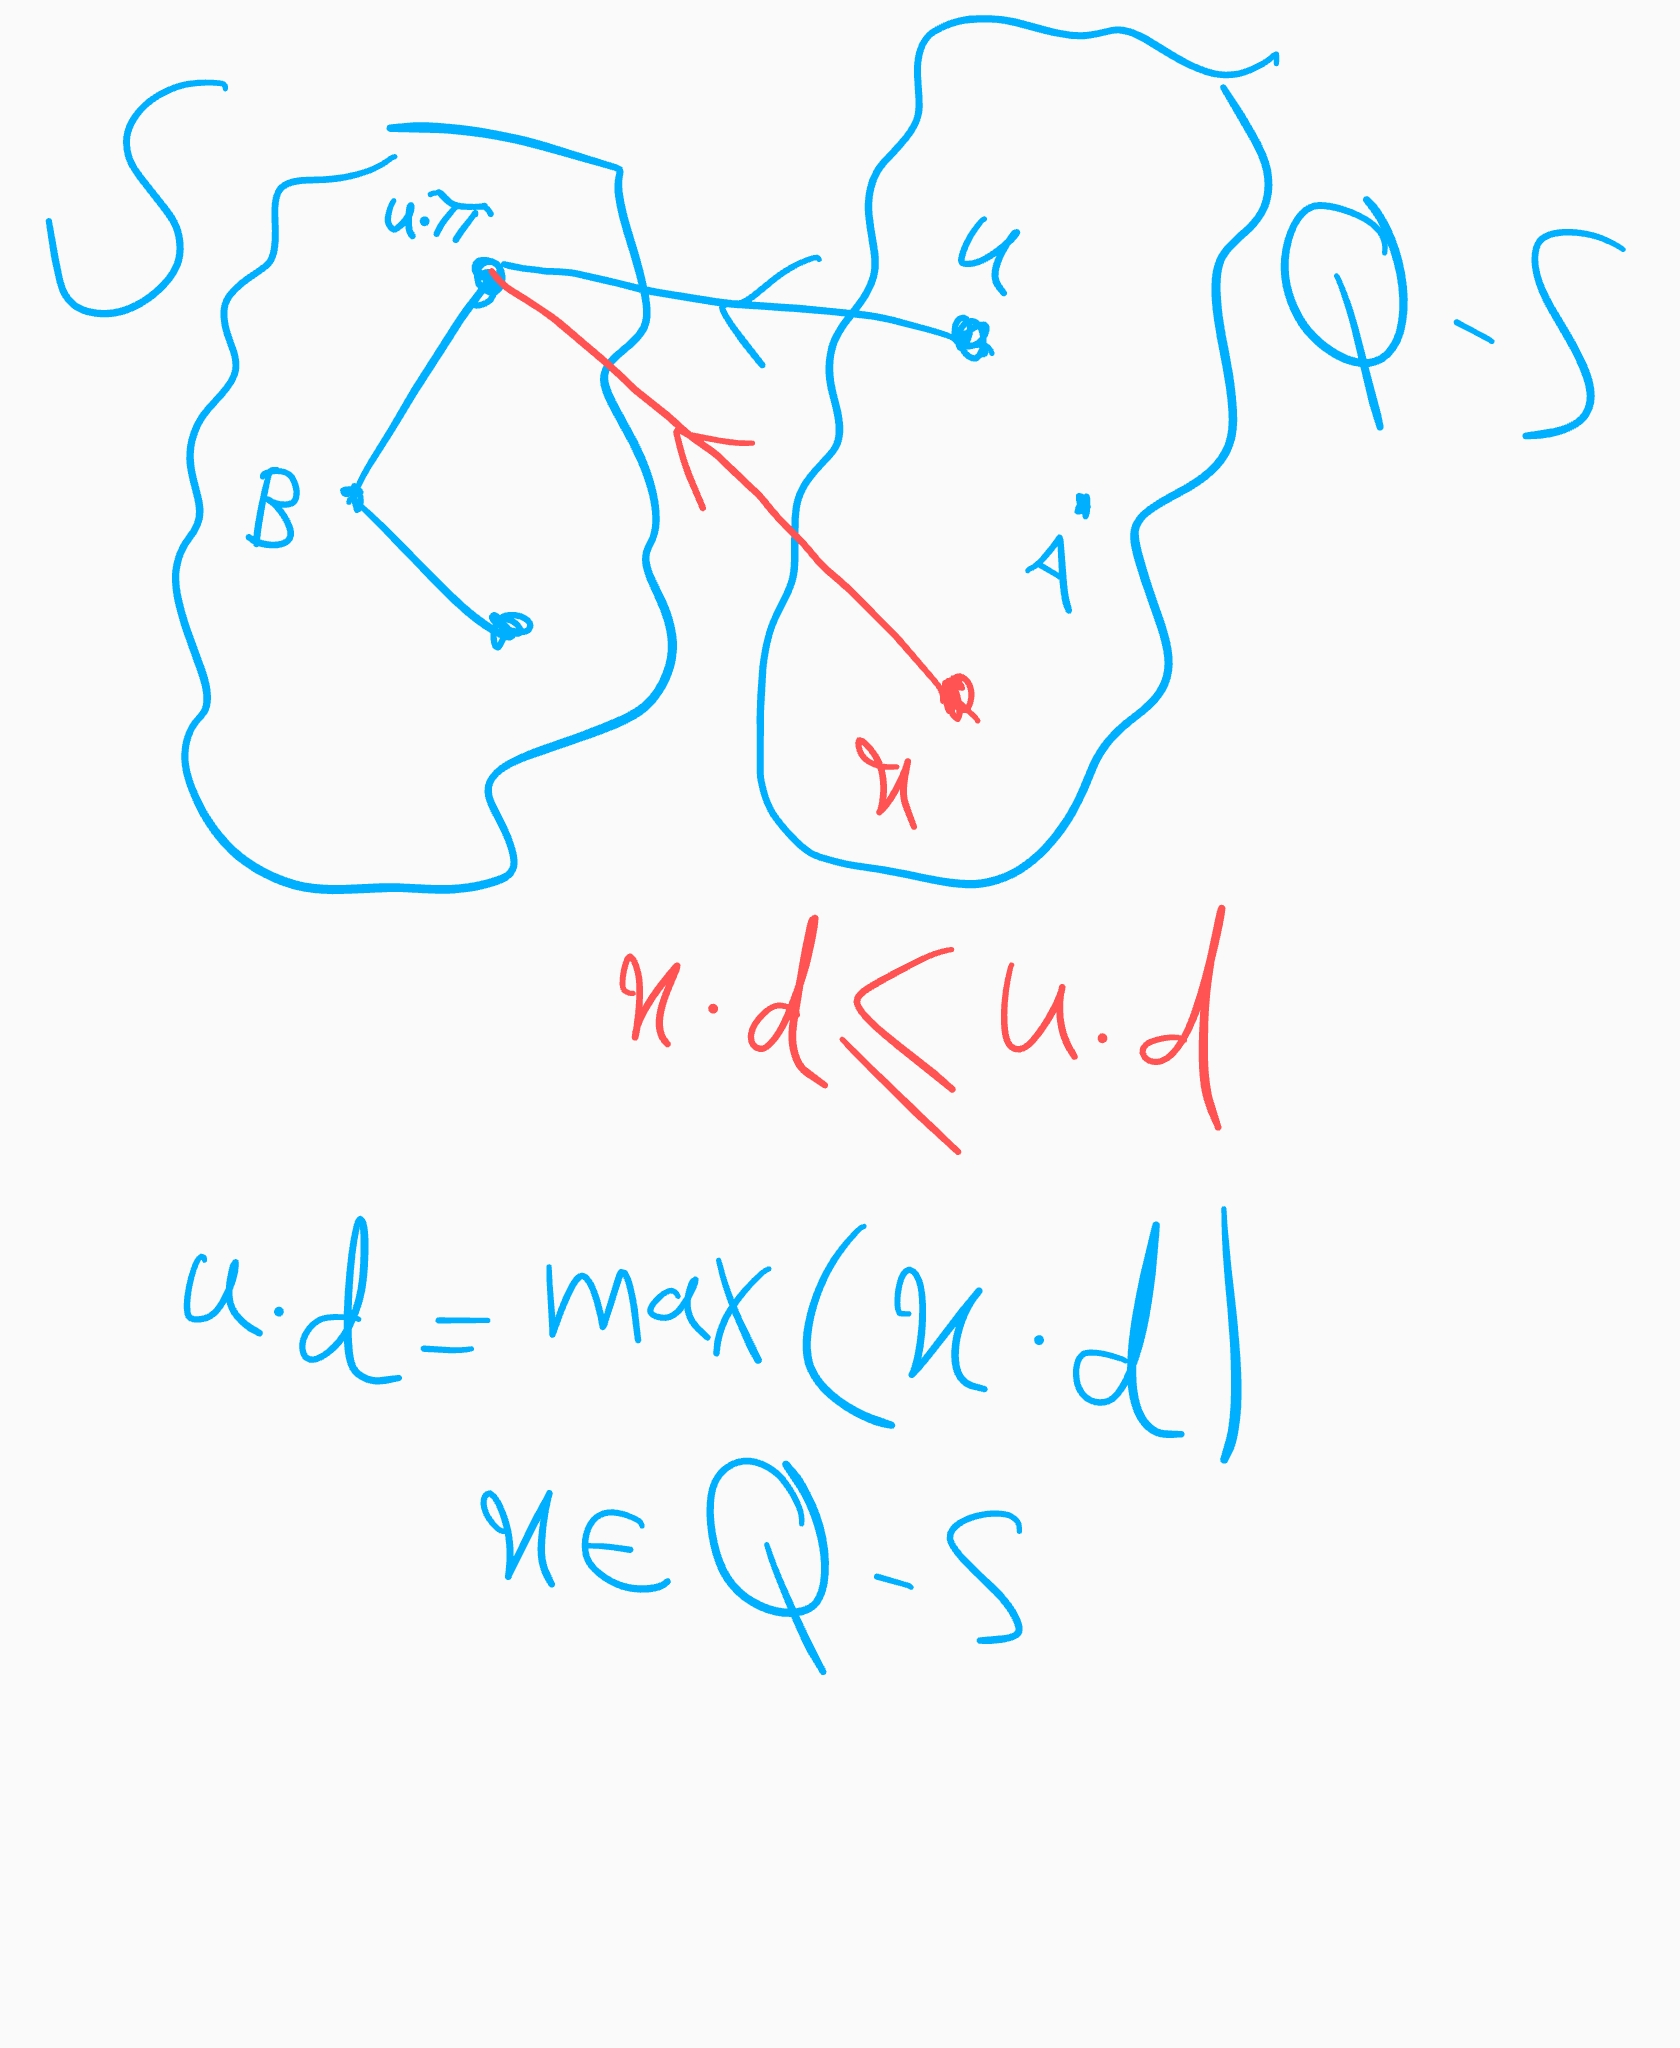
\includegraphics[width=\linewidth]{images/latest-departure.jpg}
			\end{figure}
			\begin{algorithm}[h!]
				\begin{algorithmic}[1]			
					\Function{SCHEDULING}{G, A, B, d, a, t}
						\State $G' = $ \Call{REVERSE-GRAPH-EDGES}{G}
						\State \Call{INITIALIZE-SINGLE-SOURCE}{$G'$, s}
						\State $B.d = t + 1$ \Comment To make sure we arrive at $B$ no more than $t$
						\State $S = \emptyset$
						\State $Q = G'.V$
						\While{$Q \ne \emptyset$}
							\State $u = $ \Call{EXTRACT-MAX}{$G'$}
							\State $S = S \cup \{u\}$
							\ForAll{$v \in G'.Adj[u]$}
								\State \Call{RELAX}{u, v, d, a}
							\EndFor
						\EndWhile
						\If{$A.d > -\infty$}
							\State $u = A$
							\While{$u \ne B$}
								\State \Call{PRINT}{$u, u.\pi$}
								\State $u = u.\pi$
							\EndWhile
						\Else
							\State \Call{PRINT}{$"IMPOSSIBLE"$}
						\EndIf
					\EndFunction
				\end{algorithmic}
			\end{algorithm}
			\begin{algorithm}[h!]
				\begin{algorithmic}[1]
					\Function{RELAX}{u, v, d, a}
						\If{$(a_{vu} + 1) \le u.d \land d_{vu} > v.d$}
							\State $v.d = d_{vu}$
							\State $v.\pi = u$
						\EndIf
					\EndFunction
				\end{algorithmic}
			\end{algorithm}
			\begin{algorithm}[h!]
				\begin{algorithmic}
					\Function{INITIALIZE-SINGLE-SOURCE}{G, s}
						\ForAll{$v \in G.V$}
							\State $v.d = -\infty$
							\State $v.\pi = NIL$
						\EndFor
					\EndFunction
				\end{algorithmic}
			\end{algorithm}
			\FloatBarrier			
		\end{itemize}
	\end{enumerate}
	\item \textbf{Single-pair shortest-path problem:}
	Many problems for previous sections actually belong here.
	\item \textbf{All-pair shortest-path problem:}
	\end{enumerate}
	
	\chapter{All-Pairs Shortest Path}
	For an alternative solution see exercise 5 of Bellman-Ford algorithm.
	\paragraph{Weight definition} We assume that the vertices are numbered $1, 2, \dots, |V|$, so that the input is an $n \times n$ matrix $W$ representing the edge weights of an n-vertex directed graph $G = (V, E)$. That is, $W = (w_{ij})$. Suppose $w(i, j)$ is the weight of directed edge $(i, j)$ in which $(i, j) \in E$. We define $w_{ij}$ as:
	\begin{equation*}
		w_{ij} = \begin{cases}
			0 & i = j \\
			w(i, j) & i \ne j \land (i, j) \in E \\
			\infty & i \ne j \land (i, j) \notin E
		\end{cases}
	\end{equation*}
	\section{The Floyd-Warshall algorithm}
	Let $d_{ij}^{(k)}$ be the weight of a shortest path from vertex $i$ to vertex $j$ for which all intermediate vertices are in the set $\{1, 2, \dots, k\}$:
	\begin{equation*}
	d_{ij}^{(k)} = \begin{cases}
		w_{ij} & k = 0 \\
		\min(d_{ij}^{(k - 1)}, d_{ik}^{(k - 1)} + d_{kj}^{(k - 1)}) & k \ge 1
	\end{cases}
	\end{equation*}
	Because for any path, all intermediate vertices are in the set $\{1, 2, \dots, n\}$, the matrix $D^{(n)} = (d_{ij}^{(n)})$ gives the final answer: $d_{ij}^{(n)} = \delta(i, j)$ for all $i, j \in V$.
	
		\begin{algorithm*}[h!]
			\begin{algorithmic}[1]
				\Function{Floyd-Warshall}{$W$}
					\State $n = W.rows$
					\State $D^{(0)} = W$
					\For{$k = 1$ TO $n$}
						\State let $D^{(k)} = (d_{ij}^{(k)})$ be a new $n \times n$ matrix
						\For{$i = 1$ To $n$}
							\For{$j = 1$ TO $n$}
								\State $d_{ij}^{(k)} = \min(d_{ij}^{(k - 1)}, d_{ik}^{(k - 1)} + d_{kj}^{(k - 1)})$
							\EndFor
						\EndFor
					\EndFor
				\EndFunction
			\end{algorithmic}
		\end{algorithm*}
		\FloatBarrier
	As you can see $d_{ij}^{(k)}$ is a 3-dimensional array. We can use a 2D array. We assumed $D_{ij}$ has the correct answer for intermediate vertices $1, 2, \dots, k - 1$. Now we want to add vertex $k$ as a new intermediate vertex:

		\begin{algorithm*}[h!]
			\begin{algorithmic}[1]
				\Function{Floyd-Warshall}{$W$}
					\State $n = W.rows$
					\State $D = W$
					\For{$k = 1$ TO $n$}
						\For{$i = 1$ To $n$}
							\For{$j = 1$ TO $n$}
								\If{$D_{ik} + D_{kj} < D_{ij}$}
									\State $D_{ij} = D_{ik} + D_{kj}$
								\EndIf
							\EndFor
						\EndFor
					\EndFor
				\EndFunction
			\end{algorithmic}
		\end{algorithm*}
		\FloatBarrier	
	
	\paragraph{Transitive closure of a directed graph}
	\begin{enumerate}
		\item Given a directed graph G. Design an algorithm to determine whether or not there is at least one cycle. See TopCoder SRM 705 DIV 2 question 500.
		\begin{itemize}
			\item[\textbf{Solution}] We can use DFS and if we find a back edge then it's part of a cycle. We can use transitive closure to solve this problem. We assume we don't have loop edges.
			\begin{algorithm*}[h!]
				\begin{algorithmic}
					\Function{CYCLE}{G}
						\State $n = |G.V|$
						\State let $T = (t_{ij})$ be a new $n \times n$ matrix
						\For{$i = 1$ to $n$}
							\For{$j = 1$ to $n$}
								\If{$i \ne j \land (i, j) \in G.E$}
									\State $t_{ij} = 1$
								\Else
									\State $t_{ij} = 0$								
								\EndIf
							\EndFor
						\EndFor
						\For{$k = 1$ to $n$}
							\For{$i = 1$ to $n$}
								\For{$j = 1$ to $n$}
									\State $t_{ij} = t_{ij} \lor (t_{ik} \land t_{kj})$
								\EndFor
							\EndFor
						\EndFor
						\For{$i = 1$ to $n$}
							\If{$t_{ii} == TRUE$}
								\State \Return $TRUE$
							\EndIf
						\EndFor
						\State \Return $FALSE$
					\EndFunction
				\end{algorithmic}
			\end{algorithm*}
		\end{itemize}
	\end{enumerate}
		
	\chapter{Maximum Flow}
	\chapter{Flow networks}
	\section{The Ford-Fulkerson method}
	\paragraph{Dealing with antiparallel edges}
	\subparagraph{Forbidding antiparallel edges}
	This is the approach of the textbook. Suppose flow network $G = (V, E)$. If $(u, v) \in E$, then $(v, u) \not\in E$. With this definition we always have $0 \le f(u, v) \le c(u, v)$ in which $f(u, v)$ is the flow between $(u, v)$ and $c(u, v)$ is its capacity. Based on this definition of flow network we have the following "residual capacities".
	\begin{equation}
	\label{eq:ResidualCapacityNoAntiParallel}
	c_f(u, v) = \begin{cases}
	c(u, v) - f(u, v) & (u, v) \in E \\
	f(v, u) & (v, u) \in E \\
	0 & \text{otherwise}
	\end{cases}
	\end{equation}
	Since antiparallel edges are not allowed, it is impossible that we have $(u, v) \in E \land (v, u) \in E$. So the definition of residual capacities is well defined. Given a flow network $G = (V, E)$ and a flow $f$, the \textbf{residual network} of $G$ induced by $f$ is $G_f = (V, E_f)$, where $E_f = \{(u, v) \in V \times V : c_f(u, v) > 0\}$.\\
	Now we need to deal with the flow of edges. If $f$ is a flow in $G$ and $f'$ is a flow in the corresponding residual network $G_f$, we define $f \uparrow f'$, the \textbf{augmentation} of flow $f$ by $f'$, to be a function from $V \times V$ to $\mathbb{R}$, defined by
	\begin{equation}
	\label{eq:augmentationOfFlowNoAntiparallel}
		(f \uparrow f')(u, v) = \begin{cases}
		f(u, v) + f'(u, v) - f'(v, u) & (u, v) \in E \\
		0 & \text{otherwise}
		\end{cases}
	\end{equation}
	If $f$ is a flow in $G$, the \textbf{value} of $f$ is defined as $|f| = \sum_{v \in V}f(s, v) - \sum_{v \in V}f(v, s)$ in which $s$ is the source. In the textbook it was proven that $|f \uparrow f'| = |f| + |f'|$.\\
	Consider augmenting path $p$ from source to sink. We define \textbf{residual capacity} of $p$ as $c_f(p) = \min\{c_f(u, v) : (u, v) \text{ is on } p\}$. In the textbook it was proven that the following function $f_p : V \times V \rightarrow \mathbb{R}$ is a flow in $G_f$ with value $|f_p| = c_f(p) > 0$.
	\begin{equation*}
	f_p(u, v) = \begin{cases}
	c_f(p) & \text{if } (u, v) \text{ is on } p \\
	0 & \text{otherwise}
	\end{cases}
	\end{equation*}
	So we can use $|f \uparrow f_p| = |f| + |f_p| > |f|$ to increase the flow until we reach maximum flow.
	\subparagraph{Allowing antiparallel edges}
	Suppose in flow network $G = (V, E)$ it is possible $(u, v) \in E \land (v, u) \in E$. We need to redefine some definitions. Consider Ford-Fulkerson algorithm. In each step we increase flow $f$ until we reach maximum flow. Suppose the flow of $G$ is $f_i$ in i\textsuperscript{th} step. So we have $f_1, f_2, \dots, f_m$. It is obvious $|f_1| = 0$ and $|f_m|$ is the value of maximum flow. Suppose we are in the i\textsuperscript{th} step and $p$ is an augmenting path from source to sink. The \textbf{residual capacity} in the i\textsuperscript{th} step is given by
	\begin{equation}
	\label{eq:ResidualCapacityWithAntiParallel}
		c_{f_i}(u, v) = \begin{cases}
		c_{f_{i - 1}}(u, v) - c_{f_i}(p) & (u, v) \text{ is on } p \\
		c_{f_{i - 1}}(u, v) + c_{f_i}(p) & (v, u) \text{ is on } p \\
		c_{f_{i - 1}}(u, v) & \text{otherwise}
		\end{cases}
	\end{equation}
	For the base case we have $c_{f_1} = C$ in which $C$ is the capacities for all edges. Note that equation \ref{eq:ResidualCapacityWithAntiParallel} not only is the general definition of equation \ref{eq:ResidualCapacityNoAntiParallel}, but also easier to implement. Unlike equation \ref{eq:ResidualCapacityNoAntiParallel} which required the amount of edge flow, equation \ref{eq:ResidualCapacityWithAntiParallel} only relies on previous residual capacities.\\
	Now we need to redefine equation \ref{eq:augmentationOfFlowNoAntiparallel}. Suppose $p$ is an augmenting path in the i\textsuperscript{th} step.
	\begin{equation}
		f_i(u, v) = (f_{i - 1} \uparrow f_p)(u, v) = c(u, v) - c_{f_i}(u, v)
	\end{equation}
	By this definition it is possible we have negative flow. If $f(u, v) < 0$, it means the actual flow is from $v$ to $u$. In other words, $f(v, u) > 0$. More precisely, if $f(u, v) = k$ which $k > 0$, then $f(v, u) = -k$. We can prove it through mathematical induction. At the start $|f| = 0$ which holds our assumption and we use it as our base case. Suppose in the $(i - 1)$\textsuperscript{th} step, $f(u, v) = k_{i - 1}$ and $f(v, u) = -k_{i - 1}$. We need to prove this condition holds in the step $i$. Without loss of generality suppose $(u, v)$ is on augmenting path $p$:
	\begin{equation*}
		\begin{split}
		f_i(u, v) &= c(u, v) - c_{f_i}(u, v) \\
		&= c(u, v) - [c_{f_{i - 1}}(u, v) - c_{f_i}(p)] \\
		&= k
		\end{split}	
	\end{equation*}
	\begin{equation*}
		\begin{split}
		f_i(v, u) &= c(v, u) - c_{f_i}(v, u) \\
		&= c(v, u) - [c_{f_{i - 1}}(v, u) + c_{f_i}(p)] \\
		&= -k
		\end{split}
	\end{equation*}
	It means:
	\begin{equation*}
		\begin{split}
		c(u, v) - c_{f_{i - 1}}(u, v) + c_{f_i}(p) &= -c(v, u) + c_{f_{i - 1}}(v, u) + c_{f_i}(p)\\
		\Rightarrow c(u, v) - c_{f_{i - 1}}(u, v) &= -c(v, u) + c_{f_{i - 1}}(v, u) \\
		\Rightarrow f_{i - 1}(u, v) &= -f_{i - 1}(v, u)
		\end{split}
	\end{equation*}
	So with this definition we have
	\begin{equation}
		f_i(u, v) = -f_i(v, u)
	\end{equation}
	\paragraph{Minimum cut}
	A minimum cut of a network is a cut whose capacity is minimum over all cuts of the network. Since we must respect the capacity of each edge when we calculating maximum flow, intuitively we calculated minimum cut. 
	\paragraph{Minimum cut properties}
	Suppose we have a flow network with maximum flow. Consider the final residual network $G_f$. Obviously we shouldn't have any augmenting path from $s$ to $t$.
	\begin{itemize}
		\item[] \textbf{augmenting reachable vertex u:} If there is an augmenting path from $s$ to $u$ in the final residual network $G_f$, we call $u$ augmenting reachable from $s$. Obviously $t$ is not augmenting reachable in the final residual network. So we call it augmenting unreachable
	\end{itemize}
	Consider $cut(S, T)$ in which $S$ is the set of all augmenting reachable vertices from $s$ and $T = V - S$ has all augmenting unreachable vertices from $s$. Obviously $t \in T$. Otherwise we have an augmenting path from $s$ to $t$. We have $\forall (u, v) \in \{(x, y) \in E : x \in S \land y \in T \}$:
	\begin{equation*}
	\begin{split}
	flow(u, v) &= c(u, v) \\
	c_f(u, v) &= 0 \\
	\end{split}		
	\end{equation*}
	and $\forall (a, b) \in \{(x, y) \in E : a \in T \land b \in S \}$ we have:
	\begin{equation*}
	\begin{split}
	flow(a, b) &= 0 \\
	c_f(a, b) &= c(a, b) \\
	\end{split}		
	\end{equation*}	
	$c_f(u, v)$ is residual capacity of each edge which is defined as:
	\begin{equation*}
		c_f(u, v) = \begin{cases}
		c(u, v) - f(u, v) & (u, v) \in E \\
		f(v, u) & (v, u) \in E \\
		0 & \text{otherwise}
		\end{cases}
	\end{equation*}
	Note that if $flow(a, b) > 0$, then $c_f(b, a) = flow(a, b)$ which means $a$ is augmenting reachable from $s$ which is a contradiction. Since $flow(u, v) = c(u, v)$, this is a \textbf{"minimum cut"}. This property holds weather or not anti-parallel edges are allowed. Suppose $(u, v) \in E$ and $(v, u) \in E$ and $u \in S$ and $v \in T$. Then we have:
	\begin{equation*}
		\begin{split}
		flow(u, v) &= c(u, v) \\
		flow(v, u) &= 0 \\
		c_f(u, v) &= 0 \\
		c_f(v, u) &= c(v, u)
		\end{split}
	\end{equation*}
	Note that if $c_f(u, v) > 0$ then $v$ is augmenting reachable from $s$ which is a contradiction. Hence $c_f(u, v) = 0$ which means $flow(u, v) = c(u, v)$ and $flow(v, u) = 0$. For more information you can see \href{https://www.topcoder.com/community/data-science/data-science-tutorials/maximum-flow-section-1/}{"TopCoder's Maximum Flow: Section 1"} and \href{https://www.topcoder.com/community/data-science/data-science-tutorials/maximum-flow-section-2/}{"TopCoder's Maximum Flow: Section 2"}.
	\begin{enumerate}
		\item Given a weighted directed graph $G$, remove a minimum-set of edges in such a way that a given node is unreachable from another given node.
		\begin{itemize}
			\item We convert graph $G$ to a flow network. We use the weight of edges as their capacities. So $c(u, v) = w(u, v)$. Run max flow algorithm on the flow network until we don't have any augmenting path from $s$ to $t$. Put all augmenting reachable vertices from $s$ into set $S$ and the others in $T$ to get a min cut. All edges $(u, v) \in E$ that are from $S$ to $T$ have flow $f(u, v) = c(u, v)$ and all edges $(x, y) \in E$ that are from $T$ to $S$ have flow $f(x, y) = 0$. In other words the capacity of min cut is $\sum_{u \in S}\sum_{v \in T}w(u, v)$. So by removing the crossing edges of min cut we solve the problem optimally.
		\end{itemize}
		\item Exercise 11 in \ref{sec:MaxFlowEdgeConnectivity}
	\end{enumerate}
	\subsection{Exercises}
	\paragraph{Exercise 11}
	\phantomsection
	\label{sec:MaxFlowEdgeConnectivity}
	\subparagraph{Wrong greedy appraoch} Remove all edges that are incident to a vertex with minimum degree. We need to prove this greedy choice lead to a optimal solution in general. Suppose $u$ has the minimum degree $k$. We have an optimal solution $s$ in which at least one of the edges $(u, v)$ for $v \in V - \{u\}$ is not removed. We need to prove we can convert $s$ to $s'$ which all incident edges to $u$ is removed and is optimal as $s$. Without loss of generality suppose $k = 2$ and $w$ is the isolated vertex in $s$.
	\begin{figure*}[h!]
		\centering
		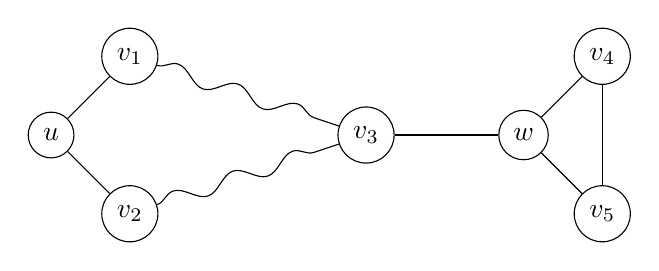
\begin{tikzpicture}
		\tikzset{vertex/.style={shape = circle, draw, minimum size = 1.5em}}
		\tikzset{snake it/.style={
				decoration={snake, 
					amplitude = 1mm,
					segment length = 8mm,
					post length=0.9mm},decorate}}
		%vertices
		\node[vertex] (u) at (0, 0) {$u$};
		\node[vertex] (v1) at (1, 1) {$v_1$};
		\node[vertex] (v2) at (1, -1) {$v_2$};
		\node[vertex] (v3) at (4, 0) {$v_3$};
		\node[vertex] (w) at (6, 0) {$w$};
		\node[vertex] (v4) at (7, 1) {$v_4$};
		\node[vertex] (v5) at (7, -1) {$v_5$};
		%edges
		\draw (u) -- (v1);
		\draw (u) -- (v2);		
		\draw (v3) -- (w);
		\draw (w) -- (v4);
		\draw (w) -- (v5);
		\draw (v4) -- (v5);			
		\path (v1) edge[snake it] (v3);
		\path (v2) edge[snake it] (v3);
		\end{tikzpicture}
	\end{figure*}
	As you can see neither $w$ nor $v_3$ have minimum degree and with removing only one edge we can make the graph disconnected.
	\FloatBarrier
	\subparagraph{Correct max flow min cut approach} We choose an arbitrary vertex $s$ as source and each $t \in V - \{s\}$ as sink. We create a new directed graph $G' = (V, E')$. $\forall (u, v) \in E$ $(u, v) \in E' \land (v, u) \in E'$. It is obvious $|E'| = 2|E|$. Then we can make a flow network form $G'$. Note that we violate the assumption if $(u, v) \in E'$, then $(v, u) \not\in E'$ for flow networks. But the algorithm still works and it's not a big deal. Also $s$ can have incoming edges and $t$ can have outgoing edges which is not violating any assumptions. We assign capacity $1$ to each edge.\\
	So we have $|V| - 1$ flow networks each of them has $s$ as its source and $t \in V - \{s\}$ as its sink. We need to find max flow in each of them and choose the minimum of them as the result. Suppose $S$ and $T = V - S$ is a min cut and $E_c = \{(u, v) \in E' : u \in S, v \in T\}$. Since each edge has capacity $1$, $\forall (u, v) \in E_c$, $flow(u, v) = 1 \land flow(v, u) = 0$, max flow is the number of edges in the min cut of that flow network. So by removing those edges in $G$ we solve the problem optimally. \\
	Generally for min cut $S$ and $T = V - S$ and $\forall (u, v) \in \{(x, y) \in E : x \in V \land y \in T \}$ we have:
	\begin{equation*}
		\begin{split}
		flow(u, v) &= c(u, v) \\
		flow(v, u) &= 0 \\
		c_f(u, v) &= 0 \\
		c_f(v, u) &= c(u, v)
		\end{split}		
	\end{equation*}
	$c_f(u, v)$ is the capacity of each edge in residual network. For more information you can see \href{https://www.topcoder.com/community/data-science/data-science-tutorials/maximum-flow-section-1/}{"TopCoder's Maximum Flow: Section 1"} and \href{https://www.topcoder.com/community/data-science/data-science-tutorials/maximum-flow-section-2/}{"TopCoder's Maximum Flow: Section 2"}.
	\paragraph{Exercise 13}
	Suppose $S$ is a cut of $V$ which $s \in S$ and $t \in V - S$. We call $T = V - S$. We define the capacity of that cut $c(S, T) = \sum_{u \in S}\sum_{v \in T}c(u, v)$. If we increase the capacity of each edge in $E$ by 1, we have $c(S, T) = \sum_{u \in S}\sum_{v \in T}{c(u, v) + 1} = \sum_{u \in S}\sum_{v \in T}{c(u, v)} + k$ which $k$ is the number of edges that cross the cut. But it's not enough. It is possible we have a cut which its capacity is not minimum but it has fewer edges than min cut. So by increasing the capacities, it'll become the new min cut. We know that $k \le E$. Hence we can define $T = E + 1$ and change the capacities as following:
	\begin{equation*}
		\begin{split}
		c(S, T) &= \sum_{u \in S}\sum_{v \in T}{T \times c(u, v) + 1} \\
		&= T \sum_{u \in S}\sum_{v \in T}{c(u, v)} + k \\
		&= Tq + k
		\end{split}
	\end{equation*}
	So even if min cut has $E$ edges, increasing its edges by $1$ is less than the other cuts which are not minimum. For more information you can see \href{https://www.topcoder.com/community/data-science/data-science-tutorials/maximum-flow-section-2/}{TopCoder's Maximum Flow: Section 2}.
\end{document}
